\documentclass[12pt,a4paper,twoside]{book}

\usepackage{graphicx}
\usepackage[utf8]{inputenc}
\usepackage[spanish,activeacute,es-tabla]{babel}
\usepackage[left=3cm,right=3cm,bottom=3.5cm,top=3.5cm]{geometry}
\usepackage{kpfonts}
\usepackage{xcolor}		
\usepackage{amsthm}
\usepackage{amsmath}
\usepackage{amssymb}
\usepackage{lipsum}
\usepackage{caption}
\usepackage{subcaption}
\usepackage{hyperref}
\usepackage{wrapfig}
\usepackage[font=small,labelfont=bf]{caption}
\usepackage{algpseudocode}
\usepackage{titlesec}
\usepackage{longtable}
\usepackage{tabularray}
\usepackage{pdflscape}

\allowdisplaybreaks
\raggedbottom

\DeclareMathOperator*{\argmin}{arg\,min}

\let\oldReturn\Return
\renewcommand{\Return}{\State\oldReturn}
\usepackage{algorithm}
\floatname{algorithm}{Algoritmo}
\renewcommand{\algorithmicrequire}{\textbf{Entrada:}}
\renewcommand{\algorithmicensure}{\textbf{Salida:}}

\algdef{SE}[FUNCTION]{Function}{EndFunction}%
   [2]{\textproc{ #1}(#2)}%\ifthenelse{\equal{#2}{}}{}{(#2)}}%
   {\algorithmicend\ \algorithmicfunction}%
\algtext*{EndFunction}
\algtext*{EndIf}
\algtext*{EndFor}
\algtext*{EndWhile}

\algnewcommand\algorithmicforeach{\textbf{for each}}
\algdef{S}[FOR]{ForEach}[1]{\algorithmicforeach\ #1\ \algorithmicdo}

\makeatletter
\newenvironment{breakablealgorithm}
  {% \begin{breakablealgorithm}
   \begin{center}
     \refstepcounter{algorithm}% New algorithm
     \hrule height.8pt depth0pt \kern2pt% \@fs@pre for \@fs@ruled
     \renewcommand{\caption}[2][\relax]{% Make a new \caption
       {\raggedright\textbf{\fname@algorithm~\thealgorithm} ##2\par}%
       \ifx\relax##1\relax % #1 is \relax
         \addcontentsline{loa}{algorithm}{\protect\numberline{\thealgorithm}##2}%
       \else % #1 is not \relax
         \addcontentsline{loa}{algorithm}{\protect\numberline{\thealgorithm}##1}%
       \fi
       \kern2pt\hrule\kern2pt
     }
  }{% \end{breakablealgorithm}
     \kern2pt\hrule\relax% \@fs@post for \@fs@ruled
   \end{center}
  }
\makeatother

\graphicspath{{img/}}
\setcounter{secnumdepth}{3}

\DefTblrTemplate{contfoot-text}{normal}{Continúa en la próxima página}
\SetTblrTemplate{contfoot-text}{normal}
\DefTblrTemplate{conthead-text}{normal}{(Continuación)}
\SetTblrTemplate{conthead-text}{normal}


\renewcommand{\And}{\textbf{and} }
\newcommand{\Or}{\textbf{or} }
\newcommand{\True}{\textbf{true} }
\newcommand{\False}{\textbf{false} }
\newcommand{\Break}{\textbf{break} }

\newcommand{\todo}[1]{{\noindent \Large \color{red}TO-DO: \textbf{#1}}}
\newcommand{\problem}[1]{\textbf{\textsc{#1}}}
\newcommand{\dist}{\textnormal{dist}}


\newtheorem{theorem}{Teorema}[chapter]
\newtheorem{lemma}{Lema}[chapter]
\newtheorem{corollary}{Corolario}[chapter]
\newtheorem{claim}{Afirmaci\'on}[chapter]
\newtheorem{proposition}{Proposici\'on}[chapter]
\newtheorem{observation}{Observaci\'on}[chapter]
\theoremstyle{definition}
\newtheorem{definition}{Definici\'on}[chapter]
\newtheorem{remark}{Observaci\'on}[chapter]
\newtheorem{problemdef}{Problema}[chapter]

%\newcommand{\theoremautorefname}{Teorema}
\newcommand{\lemmaautorefname}{Lema}
\newcommand{\corollaryautorefname}{Corolario}
\newcommand{\claimautorefname}{Afirmaci\'on}
\newcommand{\propositionautorefname}{Proposici\'on}
\newcommand{\definitionautorefname}{Definici\'on}
\newcommand{\remarkautorefname}{Observaci\'on}
\newcommand{\algorithmautorefname}{Algoritmo}

\newcommand{\optpr}[3]{
%     \optpr{NAME}{INSTANCE}{QUESTION}
\problemdef{(\problem{#1})

\textbf{Input:} #2

\textbf{Output:} #3

}
\vspace{4mm}
}

% Fuente estilo Concrete Mathematics.
%\renewcommand{\rmdefault}{pplx}

% Configuracion de hyperref
\hypersetup{colorlinks=true,linkcolor=blue,citecolor=blue}

\begin{document}

%%%% CARATULA
\def\titulo{Licenciado}

\def\autor{Nahuel Nostrala Hatz}
\def\tituloTesis{Un algoritmo basado en generación de columnas para Star Routing}
\def\runtitulo{Un algoritmo basado en generación de columnas para Star Routing}
\def\director{Javier Marenco}
\def\codirector{Juan José Miranda Bront}
\def\lugar{Buenos Aires, 2023}
\input{caratula}

%%%% ABSTRACTS, AGRADECIMIENTOS Y DEDICATORIA
\frontmatter
\pagestyle{empty}
%\begin{center}
%\large \bf \runtitulo
%\end{center}
%\vspace{1cm}
\chapter*{\runtitulo}

\noindent Consideremos el problema de \problem{Star Routing}, cuyo origen se encuentra en un trabajo anterior como un problema de caminos mínimos sobre grafos. Aquí se propone una generalización de este problema que a su vez se puede interpretar como una versión del problema de ruteo de vehículos. Dados un grafo $G = (N, E)$ y una flota de vehículos capacitados inicialmente ubicada sobre el vértice depósito $d \in N$, se quiere minimizar el costo de cubrir a un conjunto de clientes $S \subset N$ realizando únicamente circuitos cerrados sobre $G$. Lo novedoso en \problem{Star Routing} es que para cubrir a un cliente ubicado sobre un nodo $v$, no se exige que el recorrido del vehículo incluya a $v$, sino que tiene permitido pasar suficientemente cerca. En un escenario donde se modela una empresa logística que envía paquetes a domicilio utilizando una cuadrilla de vehículos, esto resulta como si cada chofer tuviera la posibilidad de estacionar en una esquina cercana a la dirección del destinatario y acercarse a entregar el envío caminando.

\problem{Star Routing} es una formulación particularmente difícil de tratar del problema de ruteo de vehículos. En esta tesis exhibimos algoritmos eficientes que lo resuelven de manera exacta. En un análisis posterior se proponen heurísticas que permiten procesar instancias más grandes, pagando el costo de prescindir de soluciones óptimas. El análisis de la calidad de la solución aproximada implica la definición de cotas para limitar el error y merece ser profundizado ya que dista de la trivialidad.

El espacio de búsqueda de los algoritmos que resuelven \problem{Star Routing} es categóricamente más grande que el de las formulaciones tradicionales de VRP y este hecho lo vuelve particularmente interesante a fines teóricos. Dado que en la literatura hasta la fecha está ampliamente aceptado que los algoritmos de generación de columnas representan una técnica eficiente para tratar problemas de ruteo de vehículos, suena razonable utilizar una formulación de estas características para \problem{Star Routing}. Es usual que la dificultad del problema y por lo tanto la mayor parte de la carga computacional se concentren en el subproblema de pricing. Es por esto que hacemos una comparación entre varias ideas de la literatura que se mostraron eficientes para resolverlo, ahora adaptadas a nuestro caso particular. Muchas de las ideas desarrolladas en esta tesis se pueden adaptar a otras formulaciones complejas de problemas de optimización combinatoria sin dificultad excesiva. 

\bigskip

\noindent\textbf{Palabras clave:} Programación Lineal Entera, Vehicle Routing Problem, Star Routing, Generación de Columnas, Pricing, Heurísticas, ESPPRC, Grafos.	


\cleardoublepage
\tableofcontents

\mainmatter
\pagestyle{headings}

\chapter{Introducción}

\problem{Star Routing Problem} es un problema de optimización combinatoria que fue introducido por Tagliavini en \cite{tagliavini}. En este trabajo vamos a generalizar esta definición, y vamos a proveer algoritmos eficientes para resolverlo en el caso general utilizando técnicas basadas en generación de columnas. Se discutirán en profundidad los algoritmos y heurísticas desarrollados, en un orden en el que tiene sentido lógico e intuitivo para el lector. La última sección es computacional y contiene un análisis sobre el rendimiento de todos los modelos. 


\section{Motivación}

Si en algún momento utilizamos alguna plataforma de e-commerce para recibir productos directamente a la puerta de nuestro hogar, es altamente probable que ésta utilice un software dedicado a optimizar las rutas para realizar los envíos. Alrededor de este tema se ha escrito mucho y con el tiempo aparecieron en la industria una gran cantidad de variantes del problema. En la literatura académica se lo conoce como problema de ruteo de vehículos, de ahora en más \problem{VRP}, por sus siglas en inglés, y no solamente se investigan algoritmos eficientes para resolverlo, sino variaciones que resuelvan casos particulares pero que puedan potencialmente simplificar significativamente el cómputo. 

El problema que vamos a resolver en esta tesis surge como una variante de la versión clásica de \problem{VRP}. Fue presentado por primera vez en \cite{tagliavini} bajo el siguiente concepto: un camión de reparto sale de un depósito y realiza envíos a un conjunto de clientes ubicados en distintos puntos de la ciudad, cuando termina de atender a todos los clientes regresa al depósito. Hasta aquí no hay nada novedoso, sin embargo, también cuenta con la característica de que el camión tiene permitido no solamente parar en la dirección exacta en la que se encuentra el destino, sino también parar en alguna de las esquinas de esta cuadra, bajar del camión y realizar a pié el recorrido desde la esquina hasta la puerta.

En una tesis anterior de la misma universidad \cite{mongi-badia} se resuelve un problema muy similar. Un conjunto de colectivos escolares parte de un garage y tiene que recoger alumnos que van a una escuela. Éstos pasan por paradas que están distribuidas por el mapa y los alumnos se tienen que acercar a alguna de las paradas. Además, existe una restricción de capacidad en los colectivos. El objetivo del problema es, como siempre, minimizar la distancia recorrida por los vehículos, en un grafo que es dirigido y pesado.

Como última idea para motivar el problema, pensemos en la siguiente situación: una plataforma de comercio electrónico entrega productos a sus clientes en puntos de entrega fijos que están distribuidos por la ciudad. Cada uno de estos puntos de entrega tiene lockers que solamente pueden ser desbloqueados por quien realizó la compra. Los clientes tienen habilitado un conjunto de puntos de entrega a los que pueden acercarse a buscar su envío, y los repartidores ahora tienen que pasar por una cantidad de puntos en el mapa mucho menor. Hay dos motivos principales por los que esperaríamos que promover esta modalidad de envío podría ser beneficioso. Desde el punto de vista teórico, al resolver el problema de enrutamiento de vehículos en un grafo con menos vértices, se esperaría una complejidad computacional mejor. Desde el punto de vista práctico, si un repartidor tiene que atender varios domicilios situados muy cerca unos de otros pero en una ciudad en la que la movilidad no es eficiente, podría resultar conveniente atender a todos en una única visita. 

Lo que tienen en común estos y más problemas es que todos van a ser abordados por los modelos y algoritmos que presentaremos en este trabajo.  


\section{El problema de ruteo de vehículos}

El problema de enrutamiento de vehículos o problema de ruteo de vehículos consiste en encontrar una ruta óptima para un vehículo o flota de vehículos que debe atender clientes distribuidos a lo largo y ancho de un mapa, sujeto a ciertas condiciones adicionales. Existe un gran número de variantes de este problema dependiendo estas restricciones suplementarias, por lo que resulta difícil dar una definición que las cubra a todas. En el caso más simple de todos, este problema es indistinguible del problema del viajante de comercio (\problem{TSP}), para el cual se han podido resolver hasta la fecha instancias de decenas de miles de nodos. Sin embargo, en las variantes más desafiantes, \problem{VRP} solo puede resolverse para grafos de 100 o 200 vértices \cite{laporte}. Por esto resulta mucho más atractivo estudiar estas variantes.

Se dice que \problem{VRP} es \emph{monovehículo} si hay un único vehículo para atender a todos los clientes y caso contrario, cuando existe una flota de vehículos, lo llamamos \emph{multivehículo}. Normalmente todos los coches tienen el mismo punto de partida, que es un nodo distinguido del grafo que llamamos \emph{depósito} y también es común que cada unidad deba finalizar el recorrido en este mismo nodo. Una de las variaciones más estudiadas del problema con múltiples vehículos es el llamado problema \emph{capacitado}, de ahora en más \problem{CVRP}, en la que todos los clientes del mapa tienen una \emph{demanda} y cada uno de los móviles tiene una \emph{capacidad}, que no debe superar la suma de las demandas de los clientes que atiende. Otra formulación que es igualmente popular es el problema con \emph{ventanas de tiempo}, usualmente denotado \problem{VRPTW}, donde cada cliente solamente puede ser atendido en un rango temporal determinado, y además de determinar la ruta más corta es preciso calcular el tiempo de partida de cada unidad de la flota. También es usual agregar restricciones del siguiente estilo: el grafo podría contener múltiples depósitos, cada coche podría realizar múltiples viajes, se podría evitar atender algunos clientes para asegurar la factibilidad del problema, se podría relajar la condición de regresar al depósito una vez finalizada la ruta, y así siguiendo podemos mencionar casi una infinidad de casos.


\section{Definición del problema}

Existen múltiples maneras de representar este problema. En este trabajo presentaremos varias en un orden en el que resulta intuitivo, de la menos general a la más general. 

Una forma que resulta inmediata para modelar este problema es representarlo sobre un grafo que tiene un vértice por cada esquina y una arista por cada calle que une dos esquinas. Digamos que $G = (N, E)$ es ese grafo. Algunas de las aristas de este grafo contienen clientes, a priori es irrelevante si hay uno o varios sobre la misma cuadra, llamemos a este conjunto de aristas $X$. Buscamos ahora un conjunto de vértices que sea un camino y que además pase por todas las aristas de $X$. Cuando se habla de que un camino (o según el caso, circuito) \emph{cubre} a una arista, quiere decir que el camino contiene a uno de los vértices que son extremos de esta arista. Naturalmente, un camino cubre a un conjunto de aristas si cubre a cada arista del conjunto. La primera definición del \problem{Star Routing Problem} que se conoce está en \cite{tagliavini} y es la siguiente:

\optpr{Single-Vehicle Road Network Star Routing}{Sea $G = (N, E)$ un grafo y $X \subseteq E$ un subconjunto de las aristas del grafo.}{El camino de $G$ de longitud mínima que cubra a $X$.}

Le asignamos el nombre \emph{road network} porque este grafo representa el mapa de una ciudad, y es de forma literal una red de carreteras, a diferencia de otras formulaciones que se exploran más adelante, donde se utilizan vértices para representar clientes.

Una idea que sigue intuitivamente es la siguiente: ¿Qué pasa si en vez de tocar estrictamente una arista, pasamos suficientemente cerca de ella, digamos a distancia no mayor a $k$? Aquí se utiliza la notación $dist(x, v)$ de la manera usual, para indicar la distancia mínima entre los vértices $x$ y $v$ sobre $G$. Por otro lado, también resulta conveniente utilizar la notación $dist(x, r)$ para referirse a la distancia de un vértice $x$ a un camino $r$, que es igual a la distancia desde $x$ hasta el nodo de $r$ más cercano a $x$. Siguiendo esto, se puede extender el concepto de que un camino \emph{cubre} una arista o conjunto de aristas de la siguiente manera:

\begin{definition}
($k-$cubrimiento de vértices).
Dados $G = (N, E)$ un grafo y $X \subseteq E$ un conjunto de aristas, se dice un camino $r$ es un $k-$cubrimiento de $X$ si para todo vértice $x \in X$ se cumple $dist(x, r) \leq k$. 
\end{definition}

Esto motiva la siguiente generalización del problema:

\optpr{Single-Vehicle $k-$Star Routing}{Sea $G = (N, E)$ un grafo dirigido y completo, $X \subseteq V$ un conjunto de aristas}{El camino mínimo que sea un $k-$cubrimiento de $X$}

Observamos que el problema original (\problem{Single-Vehicle Road Network Star Routing}) se da cuando $k=0$, ya que si $r$ cubre a cada arista $x \in X$, entonces siempre vale $dist(x, r) = 0$. 

\begin{observation}
\problem{Single-Vehicle Road Network Star Routing} es un caso particular de \problem{Single-Vehicle $k$-Star Routing} cuando $k=0$.
\end{observation}

En la bibliografía de \problem{VRP} realmente es inusual que el grafo sobre el que se resuelve el problema sea \emph{road network}. Esto tiene sentido por una cuestión cuantitativa: los algoritmos más eficientes de los que consta hasta la fecha resuelven, en un tiempo de ejecución razonable, instancias de \problem{VRP} en grafos de apenas por encima de 100 vértices \cite{laporte}. En la práctica, este número resultaría razonable si uno utiliza los vértices del grafo para representar clientes, no obstante, si uno intentara representar una ciudad moderna con nodos y ejes, incluso una pequeña localidad necesitaría un grafo varios órdenes de magnitud por encima de este número, lo cual vuelve a nuestros algoritmos, como mínimo, imprácticos.
 
Lo que debemos hacer es a partir del grafo $G$ generar un nuevo grafo $G'$ que tiene un nodo por cada cliente y cada arista representa el camino mínimo entre los respectivos clientes. El costo de cada arista de este grafo se tiene que calcular de antemano. Una forma eficiente de calcular todos los caminos mínimos de un grafo es utilizando el algoritmo de Floyd-Warshall \cite{cormen}. Notemos que $G'$ es completo, porque contiene todos los caminos mínimos entre pares de nodos, y también es dirigido, porque el camino de $u$ a $v$ no necesariamente tiene el mismo costo que de $v$ a $u$.

Este es un cambio importante en la semántica del grafo pero el problema en sí no sufre una alteración significativa:

\optpr{Single-Vehicle Clique Star Routing}{Sea $G = (N, E)$ un grafo dirigido y completo, $X \subseteq N$ un conjunto de vértices}{El camino mínimo que cubra a $X$}

La única diferencia mayor es que ahora pierde sentido que los clientes se ubiquen sobre aristas. Nótese que la definición de cobertura en este caso es ambigua, y puede interpretarse como un $k-$cubrimiento o como la definición original de \problem{Vertex Cover}.

Dado que en el desarrollo de esta tesis vamos a profundizar en la literatura de \problem{VRP}, sería conveniente adaptar la definición de nuestro problema de estudio de manera que sus variables puedan ser expresadas como es usual en este tipo de problemas. Para esto se introduce el concepto de \emph{depósito}, que es simplemente el nodo donde comienza y finaliza el camino que se busca minimizar, que ahora se vuelve un circuito. 

Para terminar de explicar el problema, vamos a agregar dos condiciones más, que son clásicas en los problemas de esta índole. En primer lugar, se dispone de un conjunto $K$ de vehículos, entonces ya no tenemos que hallar un único circuito, sino uno para cada vehículo. No es necesario utilizar la totalidad de las $|K|$ unidades, puede quedar alguno ocioso. Por otro lado, se consideran restricciones de capacidad: cada uno de estos coches de servicio tiene capacidad $Q$ fija, todos tienen la misma capacidad, y cada cliente $s$ tiene una demanda asociada $q_s$, de manera que la suma de las demandas de los clientes atendidos por un mismo vehículo bajo ningún concepto puede superar $Q$. En esencia, estamos resolviendo una instancia de \problem{CVRP} \emph{multivehículo}.

Falta una última definición antes de dar la versión del problema que vamos a resolver en este trabajo. 

\begin{definition}
    ($k$-Vecindario).
    Se denomina \emph{$k$-vecindario} de $s$, y lo notamos $\varrho_k(s)$, al conjunto de nodos de $v \in N$ tales que $\text{dist}(v, s) \leq k$.
\end{definition}

El valor de $k$ se define cuando se genera una instancia del problema, y queda fijo durante todas las etapas siguientes. Además, el lector puede advertir que el parámetro $k$ solamente se utiliza para definir los $k-$vecindarios de cada cliente $s \in N$, y luego es resignado al olvido. Con la finalidad de evitar confusiones de notación, en lo que sigue a este párrafo podemos definitivamente borrarlo de su lugar. Sabiendo que los $k$-vecindarios van a estar pre-computados, podemos bautizarlos con un nombre más descriptivo para quien resuelve el problema. 

\begin{definition}
    (Parada y conjunto de paradas asociadas a $s$).
    Dado un valor de $k$ fijo, todos los vértices $p \in N$ que pertenecen al $k$-vecindario de $s \in N$ se denominan \emph{paradas} asociadas a $s$, y se define $\varrho(s)$ como el conjunto de todas las paradas asociadas a $s$. 
\end{definition}

Con esto damos la definición final del problema que se resuelve en esta tesis.

\optpr{Star VRP}{Sea $G = (N, E)$ un grafo dirigido completo y cuyas aristas $(i, j) \in E$ tienen peso $w_{ij}$. Sea $d \in N$ un nodo distinguido  llamado depósito, $K$ un conjunto de vehículos y  $S \subseteq N \setminus \{d\}$ un conjunto de clientes. Cada cliente $s \in S$ tiene asociados un  conjunto de paradas $\varrho(s)$ y una demanda $q_s$. Todos los vehículos tienen capacidad $Q$.}{
Una asignación de rutas para la flota de vehículos, de distancia total mínima, que cubre a todos los clientes y que cumple la restricción de capacidad.}
\label{star-vrp}

Una asignación de rutas hace referencia a un conjunto que tiene a lo sumo una ruta para cada vehículo (puede haber algunos sin utilizar). El concepto de cubrir a un cliente significa exactamente que pasa por alguno de los vértices que se encuentran en su conjunto de paradas. La restricción de capacidad se entiende en el sentido clásico de \problem{CVRP}: la suma de las demandas de los clientes atendidos por un vehículo no puede superar la capacidad del mismo. 

\section{Dificultad del problema}
\label{section:complexity}

Las instancias de \problem{VRP} en sus versiones tradicionales (entre las cuales se destacan, por ejemplo, las que son con capacidades y con ventanas de tiempo) se componen de un grafo cuyos vértices son a su vez clientes distintos. Profundicemos un poco en cuanto a las diferencias con nuestra definición.

Si se cumple la desigualdad triangular y el grafo es completo, vale que todos los vehículos tienen recorridos disjuntos (no repiten nodos a excepción del depósito), pero en el caso de \problem{Star VRP}, esto no es verdad porque un coche tiene permitido pasar por una parada y atender a algunos de los nodos asociados, pero no necesariamente a todos. 

En un VRP tradicional, cada solución factible del problema es una lista ordenada de nodos que comienza en el depósito y termina en este mismo punto, aunque naturalmente no todos los circuitos simples son factibles porque pueden no satisfacer alguna de las restricciones adicionales. En \problem{Star VRP} una solución factible implica indicar la ruta que recorre el vehículo pero además el conjunto de clientes que fueron atendidos, ya que no queda unívocamente determinado. 

Una manera posible de medir la dificultad de un problema de optimización corresponde a contar la cantidad de soluciones factibles que existen. Esto provee una cota superior de la complejidad computacional del mismo, ya que un algoritmo que las enumere puede encontrar el (algún) óptimo simplemente recorriéndolas todas. Esta medida puede resultar un tanto grosera pues generalmente uno puede encontrar propiedades particulares del problema que permitan no explorar la totalidad del espacio de búsqueda. Sin embargo, solamente por el bien del argumento, vamos a emplear este criterio para comparar estos dos problemas, porque los algoritmos que los resuelven son similares entre sí.

Sea $\Omega$ el conjunto de caminos elementales del grafo que pasan por el depósito, $N$ el conjunto de nodos y $S$ el conjunto de clientes. Notemos que por definición $|S| < |N|$, aunque en algunas instancias vale $|S| \approx |N|$, mientras que $|\mathscr{P}(S)| = 2^{|S|} = \mathcal{O}(|\mathscr{P}(N)|)$ y por otro lado $|\Omega| = \mathcal{O}(|N|!)$. La notación $\mathscr{P}(S)$ hace referencia al conjunto de todos los subconjuntos de $S$. En el caso tradicional el cardinal del espacio de búsqueda está acotado por el tamaño de $|\Omega|$, pero en nuestro caso está acotado por $|\Omega \times \mathscr{P}(S)|$. Esta cota es de una magnitud superior y por lo tanto lo que uno espera que corriendo algoritmos similares en ambos, se pueda procesar una cantidad mucho menor de clientes.  


\section{Revisión de la Literatura y Estado del Arte}

El problema de enrutamiento de vehículos aparece formalmente por primera vez en 1959 en un trabajo de Dantzig \& Ramser \cite{dantzig-ramser}. Estos autores formularon un \problem{VRP} con capacidades y lo resolvieron usando una heurística basada en matchings. Hasta esta época los algoritmos estudiados eran aproximados y basados en heurísticas, una mejora de este tipo muy citada en la academia para este problema fue la de Clarke \& Wright unos 5 años posterior \cite{clarke-wright}, donde además por primera vez se incluyen múltiples vehículos. Los primeros experimentos para resolverlo de manera exacta entre los que fueron ampliamente difundidos en la comunidad científica llegarían recién una década y media después con los trabajos de Christofides, Mingozzi \& Toth en \cite{christo-mingozzi-toth} y de Christofides et al. en \cite{christo-et-al}. El primero estaba basado en algoritmos de programación dinámica y el segundo ya empleaba modelos de programación lineal. A partir de esta fecha emergió un sinnúmero de publicaciones utilizando modelos de programación matemática para resolver variaciones de \problem{VRP}, principalmente modelos de programación lineal entera, quedando claro que éste sería el principal enfoque que se daría en los años venideros. Siguiendo estas lineas, una de las aplicaciones particularmente relevante fue la de Desrosiers, Soumis \& Desrochers en 1984 \cite{desrosiers-soumis-desrochers}, donde por primera vez se incluyó un algoritmo de \emph{generación de columnas} en un modelo de programación lineal basado en Branch \& Bound para resolver explícitamente el problema de ruteo de vehículos.
  
Si se quiere una recopilación exhaustiva sobre los enfoques que sobrevivieron el paso del tiempo en el estudio formal de este problema, se puede ver en \cite{toth-vigo}. En este libro se hizo un trabajo muy completo para enumerar formulaciones eficientes del problema, las variantes clásicas que ganaron interés teórico, las técnicas y algoritmos que más éxito tuvieron y fundamentalmente un repaso sobre las publicaciones que marcaron algún hito en la historia del problema.

El concepto de \emph{Generación de Columnas} refiere a una técnica computacional aplicada a modelos de programación lineal donde hay una cantidad muy grande de variables en comparación a la cantidad de restricciones. Bajo esta suposición, el algoritmo Simplex debería evitar enumerar todas las variables cuando en cada iteración debe decidir cuál es la próxima variable que entra en la base (o bien determinar que la solución es óptima) y por lo tanto este paso se realiza resolviendo otro problema de optimización. Consta que esta idea fue propuesta por primera vez por Ford \& Fulkerson en \cite{ford-fulkerson} para resolver el \problem{Multicommodity Flow Problem}. También Dantzig \& Wolfe desarrollan una idea para extender un programa lineal por columnas en \cite{dantzig-wolfe} utilizando un problema de optimización para la fase de pricing. Sin embargo, la primera implementación eficiente que se conoce, se utilizó para resolver el \problem{Cutting Stock Problem} por Gilmore \& Gomory, publicado en 1961 \cite{gilmore-gomory1} y continuado en 1963 \cite{gilmore-gomory2}, y dado que este algoritmo resultó mucho mejor que el existente hasta la fecha, se podría considerar éste como el punto inicial de la gran trayectoria de publicaciones sobre este tópico. 

La definición de generación de columnas implica que en cada iteración del algoritmo Simplex se resuelve un subproblema de optimización para elegir una variable para entrar en la base. En el caso particular de la mayoría de los problemas que derivan de \problem{VRP}, se modela con el \emph{Problema del Camino Mínimo Elemental con Restricciones de Recursos} (\problem{ESPPRC} en inglés), que es NP-hard en su definición general aunque han sido publicados algoritmos pseudo-polinomiales para resolver su relajación \cite{christo-et-al}. Es un problema sobre un grafo donde los clientes tienen una cantidad de recursos que se consumen en cada visita. Las restricciones de recursos indican que ninguna solución factible puede superar el límite de disponibilidad de cada recurso. Además, cada solución debe ser un camino elemental (sin nodos repetidos) entre dos vértices fijos. Diferentes enfoques se han propuesto para abordar este problema eficientemente. En este trabajo nos centraremos en dos en particular. En 2006, Righini \& Salani propusieron un algoritmo de \emph{búsqueda bidireccional} de tipo meet-in-the-middle para aprovechar condiciones de simetría que se encuentran en la mayoría de los grafos de \problem{VRP} \cite{righini-salani}. En 2016 Lozano, Duque \& Medaglia desarrollaron un algoritmo \emph{basado en pulsos}, que es en esencia un backtracking clásico de búsqueda por profundidad, pero lo novedoso es que proponen reglas de pruning que son eficientes \cite{lozano-duque-medaglia}. Revisitaremos estos algoritmos más adelante.

\section{Contenidos de la Tesis}

Una vez presentado y bien definido el problema, se dan varios algoritmos y modelos eficientes que lo resuelven, y más adelante se discuten algunas heurísticas que pueden mejorar el rendimiento. 

El primer modelo que se introduce es el llamado \emph{Modelo Compacto}, un modelo de programación lineal entera que surge naturalmente cuando se decide emplear esta técnica para representar el problema, y si bien su performance no es muy buena, como se detalla en el Capítulo \ref{ch:experiments}, tiene sentido comparar este modelo con los demás para justificar el uso de generación de columnas.

En contraste a este, presentamos un modelo extendido sobre el cual se aplicará un algoritmo de generación de columnas. En este caso queda determinado el subproblema de pricing que se puede modelar como un caso particular del \problem{ESPPRC}, y para eso proveemos tres algoritmos diferentes que resuelven este problema, todos inspirados en formulaciones que fueron exitosas en la literatura. 

En lo que viene profundizamos sobre estos tres enfoques que resuelven el pricing. El primero consiste en un modelo de programación lineal entera al cual no le aplicamos ninguna optimización. Luego tenemos un algoritmo basado en la publicación de Lozano, Duque \& Medaglia \cite{lozano-duque-medaglia} que bautizamos como algoritmos \emph{por pulsos}, para el cual adaptamos las heurísticas de poda que se proponen y posteriormente extendemos y refinamos algunas de estas ideas. El tercer modelo corresponde a un algoritmo de labeling basado en el estudio de Righini \& Salani en \cite{righini-salani}, y en este caso se investigan estructuras de datos eficientes para la implementación como así también varias heurísticas propias. 

A modo de complemento, se presentan dos heurísticas sobre el algoritmo maestro de generación de columnas que son compatibles con cualquier formulación del pricing. Por un lado introducimos el concepto de generación de columnas en dos pasos, que en cada iteración, luego de correr el pricing, intenta ''reacomodar'' las columnas ya generadas con el objetivo de reducir el número total de iteraciones. Además, revisitamos una idea utilizada en la literatura para detener la ejecución de manera temprana, provista una buena cota para el error de la función objetivo.

En el último capítulo ponemos a prueba nuestros algoritmos en instancias reales, y evaluamos el rendimiento de cada uno a través de varias métricas, y también la calidad de las soluciones obtenidas, lo cual cobra sentido especialmente para algoritmos que no son exactos. Al finalizar se da una discusión sobre los resultados obtenidos.

\cleardoublepage
\chapter{Modelos y Algoritmos}
\label{chapter:algoritmos}

En esta sección vamos a resolver el problema \problem{Star VRP}, tal como lo definimos en \ref{star-vrp}.

A lo largo de esta sección se intentará ofrecer una notación que sea consistente con la literatura en general, tarea que es por naturaleza irrealizable ya que no hay ningún estándar o convención que lo regule. Lo que sí garantizamos es que va a ser consistente durante todo este escrito.

Si bien fue explicado en detalle en \ref{star-vrp}, por motivos de practicidad a continuación vamos a recordar los parámetros que se utilizarán en todas las secciones de este capítulo. El problema se compone de los siguientes elementos:

\begin{itemize}
    \item Un grafo dirigido y completo $G = (N, E)$.
    \item El conjunto de vehículos disponibles es $K$.
    \item Un nodo distinguido $d \in N$ llamado \emph{depósito}.
    \item Un conjunto de clientes $S \subseteq N \setminus \{d\}$.
    \item Un valor de \emph{capacidad}, denominada $Q \in \mathbb{Z}^{+}$, que es igual para todos los vehículos.
    \item  $q_s \in \mathbb{Z}^{+}$ la \emph{demanda} asociada al cliente $s$.
    \item Un \emph{conjunto de paradas} $\varrho(s) \subseteq N$ para cada cliente $s$, que es el conjunto de vértices desde las cuales se lo puede atender. Vamos a utilizar como convención que $s \in \varrho(s)$.
    \item El peso de cada arco $(i, j) \in E$ se nota $w_{ij}$.
\end{itemize}

El objetivo del problema es obtener un conjunto de rutas que tenga suma mínima, donde el costo de una ruta es la suma de los pesos de sus aristas, y que cumpla las siguientes condiciones:

\begin{itemize}
\label{list:restrictions}
    \item Las rutas son circuitos en el grafo que pasan por el depósito $d$.
    \item Hay a lo sumo tantas rutas como vehículos. Se asigna una ruta a un vehículo (puede haber vehículos sin asignar).
    \item Todos los clientes son atendidos por exactamente un vehículo. Para atender a un cliente $s$, un vehículo debe pasar por alguno de los nodos de $\varrho(s)$.
    \item La suma de las demandas de los clientes atendidos por un vehículo no excede su capacidad.
\end{itemize}

Notemos que se prohíbe que el depósito contenga un cliente, la razón fundamental de esto no es más que practicidad, más adelante queremos evitar que una ruta vacía sea válida, y porque realmente, en términos del lenguaje del problema, no restringe casos interesantes. Esto prueba que $|S| \leq |N|-1$. También utilizamos la convención de que todos los clientes son a su vez paradas (esto es, $s \in \varrho(s)$). 

Ya estamos en condiciones de pasar a la parte más interesante de la tesis, donde se presentan los modelos.


\section{Modelo Compacto}
\label{section:compacto}

El siguiente modelo presenta una cantidad polinomial de variables y restricciones. A los modelos que cumplen esta condición a menudo se los conoce como \emph{modelos compactos} \cite[p.3]{lancia-serafini}.

El modelo intenta encontrar un conjunto de circuitos dirigidos que sean subgrafos de $G$ y que pasen por el depósito. Cada uno de ellos tiene asociado un conjunto de clientes que debe atender y la demanda total de este conjunto no puede superar la capacidad $Q$. La formulación que damos a continuación se basa en esta idea: en cualquier grafo dirigido, un circuito elemental es un subgrafo cuyos vértices tienen todos grado de entrada $d_{in} = 1$ y grado de salida $d_{out} = 1$, y además es fuertemente conexo. Por otro lado, se define \emph{subtour} como un circuito del subgrafo que no pasa por $d$. Para corroborar que este subgrafo sea fuertemente conexo es condición necesaria y suficiente que no existan subtours. En el caso en el que $G$ es un grafo completo, podemos utilizar una serie de restricciones lineales para romper estos subtours, conocidas como \emph{condiciones de Miller-Tucker-Zemlin (MTZ)}.  

\begin{equation}
    \min \sum_{i \in N} \sum_{j \in N} \sum_{k \in K} w_{ij} x_{ijk}
\end{equation}
Sujeto a:
\begin{align}
    \sum_{j \in N, (i, j) \in E}{x_{ijk}} = \sum_{j \in N, (j, i) \in E}{x_{jik}} \qquad & \forall {i \in N, k \in K} \label{eq:compact1} \\
    \sum_{k \in K} y_{sk} = 1 \qquad & \forall {s \in S} \label{eq:compact2} \\
    \sum_{j \in N, (d, j) \in E}{x_{djk}} = 1 \qquad & \forall {k \in K} \label{eq:compact3} \\ 
    y_{sk} \leq \sum_{i \in N}\sum_{v \in \varrho(s)}{x_{ivk}} \qquad & \forall {k \in K, s \in S} \label{eq:compact4} \\
    \sum_{s \in S}{y_{sk}q_s} \le Q \qquad & \forall {k \in K} \label{eq:compact5} \\
u_{ik} - u_{jk} + (|N| - 1)x_{ijk} \leq (|N| - 2)  \qquad & \forall {i \in N, j \in N, k \in K: i,j \neq d, j \neq i} \label{eq:compact6} \\
1 \leq u_{ik} \leq |N| - 1  \qquad & \forall {i \in N, k \in K: i \neq d} \label{eq:compact7} \\
x_{ijk} \in \{0, 1\} \qquad & \forall {i \in N, j \in N, k \in K} \label{eq:compact8} \\
y_{sk} \in \{0, 1\} \qquad & \forall {s \in S, k \in K} \label{eq:compact9}\\
u_{ik} \in \mathbb{Z}^{+} \qquad & \forall {i \in N, k \in K} \label{eq:compact10}
\end{align}

La semántica de las variables es la siguiente: $x_{ijk} = 1$ si y sólo si el vehículo $k$ pasa por el eje $(i, j) \in E$. Por otro lado $y_{sk}$ se interpreta como que el cliente $s$ es atendido por el vehículo $k$. Estas variables \emph{de servicio} se precisan porque el camino de cierto vehículo podría pasar por el cliente pero no atenderlo, por ejemplo, por no tener suficiente capacidad. La clase de variables $u_{ik}$ se utiliza solamente para expresar las condiciones MTZ, y cumplen que $u_{jk} > u_{ik}$ si el vehículo $k$ visita $j$ después de visitar $i$, y ambos son diferentes al depósito. 

La ecuación \ref{eq:compact1} garantiza que la cantidad de vehículos que entra al nodo $i$ sea la misma cantidad que sale del nodo $i$. Como explicamos, eso es necesario para que la ruta sea un ciclo. Luego \ref{eq:compact2} asegura que cada cliente es atendido por un y sólo un vehículo. La restricción \ref{eq:compact3} sirve para obligar a cada ruta a pasar por el nodo depósito $d$. La inecuación \ref{eq:compact4} muestra que un cliente $s$ solamente puede ser atendido por el vehículo $k$ si $k$ pasa por alguna parada asociada a $s$, o sea, un nodo $v \in \varrho(s)$. Es importante ver que un vehículo podría visitar a un cliente y sin embargo no atenderlo. La restricción de capacidad se expresa en \ref{eq:compact5}. Por último, \ref{eq:compact6} y \ref{eq:compact7} son las condiciones MTZ para romper subtours.

\section{Generación de Columnas}

En esta sección definimos el modelo extendido sobre el cual aplicaremos un algoritmo de generación de columnas. Para eso comenzamos con una definición que será útil:

\begin{definition}
    (Ruta factible de $G$).
    Llamamos \emph{ruta} de $G$ a un par $r = (C_r, \tilde{S}_r)$ donde $C_r$ es un camino conexo elemental (no repite vértices) de $G$ y $\tilde{S}_r \subseteq S$ un conjunto de clientes visitados por $r$. La ruta $r$ se llama \emph{factible} si $C_r$ es un circuito cerrado que pasa por el depósito $d$ y tanto $C_r$ como $\tilde{S}_r$ cumplen las restricciones del problema.
\end{definition}

Tenemos que introducir algunos parámetros que se usarán a continuación. El conjunto $\Omega$ contiene a todas las rutas factibles. Si $r = (C_r, \tilde{S}_r) \in \Omega$, el parámetro $a_{sr} \in \{0, 1\}$ indica si $s \in \tilde{S}_r$, y el parámetro $c_r$ es el costo del circuito $C_r$. 

En la siguiente subsección damos un modelo de programación lineal entera que representa el problema que queremos resolver.

\subsection{Modelo de Set Partitioning}
\label{section:set-partitioning}

\begin{equation}
    \min \sum_{r \in \Omega} c_r  \theta_r
\end{equation}
Sujeto a:
\begin{align}
    \sum_{r \in \Omega} {a_{sr}\theta_r} = 1
\qquad & \forall {s \in S} \label{eq:master1} \\
\sum_{r \in \Omega}{\theta_r} \leq |K| & \label{eq:master2} \\
\theta_r \in \{0, 1\} \qquad & \forall{r \in \Omega}
\end{align}

Las variables binarias $\theta_r$ representan que la ruta $r \in \Omega$ es parte de la solución óptima. Por como definimos $\Omega$, solamente es necesario tomar a lo sumo $|K|$ rutas de este conjunto y asignar una a cada vehículo (pueden quedar vehículos sin utilizar). 

Cada cliente $s$ tiene que ser atendido por un único vehículo, o sea que las rutas deben ser disjuntas en cuanto a los clientes que atienden (no necesariamente en cuanto a los nodos que visitan), y eso se garantiza en \ref{eq:master1}. Finalmente \ref{eq:master2} fuerza que no se elijan más rutas que vehículos disponibles.

\subsection{Restricted Master Problem}
\label{section:rmp}

El lector puede sospechar que si bien el modelo anterior es válido y la solución es exacta, calcular el conjunto $\Omega$ está lejos de ser trivial y aún si nos fuera dado por un oráculo, la cantidad de rutas factibles en él es tal que resultaría, como mínimo, desesperanzador. Llamaremos al modelo de programación lineal de la Sección \ref{section:set-partitioning} el \emph{Problema Maestro}. A continuación se presenta una forma astuta de encararlo.

Sea $\tilde{\Omega} \subset \Omega$ un subconjunto de las rutas factibles  tal que $|\tilde{\Omega}| \ll |\Omega|$. Se define el \emph{Problema Maestro Restringido}, a partir de ahora \problem{RMP}, como un modelo idéntico al Problema Maestro pero en el cual reemplazamos $\Omega$ por $\tilde{\Omega}$ y así acotamos fuertemente la cantidad de variables $\theta_r$. 

\begin{equation}
    \min \sum_{r \in \tilde{\Omega}} c_r  \theta_r
\end{equation}
Sujeto a:
\begin{align}
    \sum_{r \in \tilde{\Omega}} {a_{sr}\theta_r} = 1
\qquad & \forall {s \in S} \label{eq:rmp1} \\
\sum_{r \in \tilde{\Omega}}{\theta_r} \leq |K| & \label{eq:rmp2} \\
\theta_r \in \{0, 1\} \qquad & \forall{r \in \tilde{\Omega}}
\end{align}

Observemos que la gran mayoría de las rutas de $\Omega$ son rutas \emph{malas}, en el sentido de que son factibles pero no son razonables y no tienen verdaderas chances de ser consideradas como parte de la base. Entonces suena razonable restringir $\tilde{\Omega}$ a un conjunto de rutas \emph{buenas} y resolver un problema más chico, a pesar de que, a priori, podríamos sacrificar la exactitud del problema. El algoritmo de generación de columnas nos permitirá resolver con exactitud la relajación lineal del Problema Maestro resolviendo solamente algunas instancias del Problema Maestro Restringido. Usualmente se complementa esta idea con un algoritmo de Branch \& Price \cite{branch-and-price-source}, si estamos interesados en encontrar el óptimo exacto (es decir, el óptimo del Problema Maestro con restricciones de integralidad y no de la relajación lineal), lo cual queda vacante en esta tesis.	

En cada iteración del algoritmo Simplex existe una fase donde se evalúan los costos reducidos de todas las variables y se elige el menor para insertar esa variable en la base. Cada costo reducido se calcula como $\bar{c}_r = c_r - \lambda^{T}a_r$ donde $\lambda$ es el vector de variables duales, $c_r$ es el costo de la ruta $r$ y $a_r$ es la columna de coeficientes asociados a la variable $r$ en el modelo de Set Partitioning \ref{section:set-partitioning}. Se puede demostrar que introducir en la base una variable $\theta_r$ de costo reducido negativo garantiza que en la próxima iteración de Simplex se obtendrá una solución mejor, y más aún, que si no existen costos reducidos negativos, el problema está resuelto a optimalidad \cite{chvatal1983linear}. Supongamos que resolvimos el \problem{RMP}, cuya solución trivialmente también es factible en el Problema Maestro. Si algún costo reducido es negativo, podemos agregar esta variable a $\tilde{\Omega}$ y lo volvemos a resolver; si no existen tales, ya habremos encontrado el óptimo del Problema Maestro. El proceso de encontrar nuevas variables para agregar a $\tilde{\Omega}$ e iterar hasta que no queden más es lo que se conoce como \emph{Generación de Columnas}.

El problema aún persiste, porque calcular \emph{todos} los costos reducidos explícitamente implica hacer una operación por cada variable de $\Omega$, y eso es inaceptable. Necesitamos conseguir una manera eficiente de saber cuál es el menor $\bar{c}_r$ sin tener que calcularlos a todos explícitamente. Este problema se conoce como \emph{subproblema de pricing}. La fortaleza de generación de columnas por lo general subyace en que exista una formulación relativamente eficiente para resolver el pricing.

\begin{algorithm}[H]
    \caption{Algoritmo de generación de columnas}
    \label{al:column-generation}
    \begin{algorithmic}[1]
        \Require Una instancia del Problema Maestro. 
        \Ensure El óptimo $\Theta^{*}$ de la relajación lineal del Problema Maestro. 
        \State Sea $\Theta = \{\theta_1 = 1, \dots, \theta_k = 1\}$ una solución factible inicial
        \If{$\Theta = \emptyset$}
            \Return Problema infactible
        \EndIf
        \State $\tilde{\Omega} \gets \Theta$
        \While{ \textbf{true} }
            \State Resolver \problem{RMP} y su dual, restringidos a $\tilde{\Omega}$
            \State Sea $\Theta^{*}$ el óptimo del \problem{RMP}.
            \State Sea $\lambda$ el vector de variables duales.
            \State Resolver subproblema de pricing.
            \State $r^{*} \gets \argmin_{r \in \Omega}{\bar{c}_r}$ // $r^{*}$ es la ruta con menor costo reducido
            \If{$\bar{c}_{r^{*}} \geq 0$}
            	\Break
            \EndIf
            \State $\tilde{\Omega} \gets \tilde{\Omega} \cup \{\theta_{r^{*}}\}$
        \EndWhile
        \Return $\Theta^{*}$
    \end{algorithmic}
\end{algorithm}

El Algoritmo \ref{al:column-generation} requiere que comencemos resolviendo el \problem{RMP} con un $\tilde{\Omega}$ válido, para luego calcular las variables duales que necesita el problema de pricing. No existe hasta donde sabemos una manera mecánica de elegir este conjunto. Para que el \problem{RMP} resulte al menos factible, se precisa una heurística que provea una solución factible inicial. No es crítico en este paso que la solución esté demasiado cerca del óptimo, por lo que se priorizarán heurísticas rápidas. Proveemos una heurística en la Sección \ref{section:initial-solution-heuristic}, sin embargo, ésta podría reportar que no existen soluciones factibles cuando sí las hay, y en ese caso en \ref{feasibility-problem} damos un algoritmo infalible aunque mucho más lento.

Desrochers et al. discuten en \cite{desrochers1992} si conviene modificar levemente el \problem{RMP} para aliviar la fase de pricing. La igualdad en \ref{eq:rmp1} se reemplaza por una desigualdad que no descarta soluciones factibles pero que resulta computacionalmente menos costosa:

\begin{equation}
\label{eq:ge-restriction-rmp}
     \sum_{r \in \tilde{\Omega}} {a_{sr}\theta_r} \geq 1
\qquad \forall {s \in S}
\end{equation}

Esto se interpreta como que cada cliente debe ser atendido por uno o más vehículos. Notemos que una solución factible de este problema modificado que no es factible en el original solamente tiene clientes repetidos (atendidos por múltiples vehículos), lo cual no cambia el valor de la función objetivo.

En el ejemplo de \cite{desrochers1992} la ganancia es clave: el problema de pricing ahora no requiere que los caminos sean elementales y la solución sigue siendo factible. En nuestro caso tenemos una complicación extra, porque la nueva formulación admite clientes repetidos y eso contradice una condición del problema, entonces surge la necesidad de agregar una fase de post-procesamiento de la solución, para eliminarlos.


\subsection{Problema dual}

Será útil calcular el problema dual de la relajación lineal del Restricted Master Problem. Esto nos servirá más adelante para calcular los costos reducidos de las variables del \problem{RMP}. 
Dado que éste tiene $|S| + 1$ desigualdades, en el dual hay $|S| + 1$ variables, que las llamaremos $\lambda_s$ para $s \in \{0, \dots, |S|\}$. Utilizamos la siguiente convención: $\lambda_0$ es la variable dual asociada a \ref{eq:rmp2} y $\lambda_{s}$ es la variable asociada al $s-$ésimo cliente de $S$ de \ref{eq:rmp1}.
\\

\begin{equation}
    \max \sum_{s \in S} \lambda_s + |K| \lambda_0 
\end{equation}

Sujeto a:

\begin{align}
    \lambda_0 + \sum_{s \in S} {a_{sr} \lambda_s} \leq c_r \qquad & \forall {r \in \Omega} \\
\lambda_s \in \mathbb{R} \quad \text{libre}
\qquad &\forall {s \in S} \\
\lambda_0 \geq 0 &
\end{align}

Cabe aclarar que si en el \problem{RMP} se utiliza la desigualdad \ref{eq:ge-restriction-rmp} en lugar de la igualdad \ref{eq:rmp1}, el problema dual permanece igual salvo por que la clase de variables $\lambda_s$ cambia su rango a $\lambda_s \leq 0$. 


\subsection{Heurística para una solución inicial}
\label{section:initial-solution-heuristic}

El algoritmo de generación de columnas necesita que en cada iteración tengamos una solución factible del Problema Maestro, incluida la primera, que luego es utilizada por el subproblema de pricing. Por eso desarrollamos una heurística que encuentra una asignación de rutas factible para \problem{Star VRP}.

Esta heurística depende fuertemente del hecho de que $G$ es completo. Vamos a empezar con una definición.

\begin{definition}
    (Partición factible de clientes).
    Una partición de $S$ en $n$ subconjuntos $\{S_1, \dots, S_n\}$ se llama \emph{factible} si estos son disjuntos dos a dos, su unión es $S$, y se cumple que $\sum_{s \in S_i} q_s \leq Q$ para todo $1 \leq i \leq n$, es decir, que la suma de las demandas en cada subconjunto no supera la capacidad.
\end{definition}

Como el grafo es completo, siempre existe un circuito que parte del depósito, recorre todos los vértices de $S_i$ en algún orden y vuelve al depósito. Esto ya nos da una idea de cómo va a ser el algoritmo, aunque nos falta ver algo más. 

\begin{definition}
    (Partición minimal y mínima de clientes).
    Una partición factible de $S$ se dice \emph{minimal} si no existen dos subconjuntos $S_i, S_j$ tales que $\sum_{s \in S_i \cup S_j} q_s \leq Q$. Se dice que esta partición es \emph{mínima} si no existe una partición minimal de cardinal menor.
\end{definition}

Si tenemos una partición factible de clientes de tamaño $n$ y se cumple que $n \leq |K|$, el problema quedaría resuelto, ya que vimos cómo construir una ruta para cada uno de estos conjuntos. Primero veremos una heurística eficiente para encontrar esta partición. El caso en el que $n > |K|$ es difícil de tratar y será estudiado más adelante. Observemos además que si el problema no es factible, no existe tal partición de clientes.

\begin{observation}
    \label{obs:heuristic-observation}
    \problem{Star VRP} es factible si y sólo si existe una partición factible mínima de clientes de tamaño a lo sumo $|K|$.
\end{observation}

Proponemos dividir la heurística en dos partes: un algoritmo que construye una partición factible minimal y otro que crea los circuitos a partir de la partición.

\begin{algorithm}[H]
  \caption{Algoritmo para construir una partición factible minimal}
  \label{al:feasible_minimal_partition_algorithm}
  \begin{algorithmic}[1]
  	\Require $S$ un conjunto de clientes.
  	\Ensure Una partición factible minimal $\mathscr{P}$.
        \State $\text{demanda} \gets 0$
        \State $i \gets 0$
        \ForEach {$s \in S$}
            \State $\text{demanda} \gets \text{demanda} + q_s$
            \If {$\text{demanda} > Q$}
                \State $i \gets i + 1$
                \State $\text{demanda} \gets q_s$
            \EndIf
            \State $S_i = S_i \cup \{s\}$
        \EndFor
        \State $n \gets i$
	\Return $\mathscr{P} = \{S_1, \dots, S_n\}$
  \end{algorithmic}
\end{algorithm}

El primer algoritmo nos garantiza encontrar una solución minimal, aunque no necesariamente mínima. El segundo algoritmo es heurístico y da como resultado la solución factible que necesitamos. Toma como parámetro el resultado del algoritmo anterior. Es importante notar que si $n > |K|$ no podemos utilizarlo, y tenemos que proceder como se explica en \ref{feasibility-problem}.

\begin{algorithm}[H]
  \caption{Heurística para construir una solución factible.}
  \label{al:feasible_solution_heuristic}
  \begin{algorithmic}[1]
  	\Require $\mathscr{P}$ una partición factible minimal de clientes.
  	\Ensure Un conjunto de rutas que cumple las restricciones de \problem{Star VRP}.
        \ForEach{$S_i \in \mathscr{P}$}
            \State $\text{ruta}_i \gets \emptyset$
            \State $\text{AgregarNodo(ruta}_i \text{, } d \text{)}$
            \ForEach{$v \in S_i$}
                \State $\text{AgregarNodo(ruta}_i \text{, } v \text{)}$
            \EndFor
            \State $\text{AgregarNodo(ruta}_i \text{, } d \text{)}$
        \EndFor
	\Return $\{\text{ruta}_1, \dots, \text{ruta}_n\}$
  \end{algorithmic}
\end{algorithm}

En este problema se tomó la decisión de que no es necesario utilizar los $|K|$ vehículos. Sin embargo, si este no fuera el caso, el algoritmo se puede adaptar fácilmente: si $n = |K|$, no hay nada que hacer, y si $n < |K|$, entonces tenemos que romper la condición de minimalidad. Basta con tomar un subconjunto cualquiera $S_i \in \mathscr{P}$ y hacerlo atravesar una suerte de mitosis que haga resultar dos conjuntos en lugar de uno. Llamemos $\mathscr{P'}$ a la nueva partición, entonces queda $S_i = S_i \setminus \{s\}$ y se crea un nuevo conjunto $S_{n+1} = \{s\}$, de manera que $|\mathscr{P'}| = |\mathscr{P}| + 1$. Realizamos este proceso hasta que la partición resultante tenga el tamaño buscado.

Es importante aclarar que esta heurística puede no encontrar soluciones factibles en caso de haberlas, y si esto llegase a ocurrir estamos obligados a correr otro algoritmo que resuelve este problema, que se detalla en la próxima sección.


\subsubsection{Problema de factibilidad}
\label{feasibility-problem}

En la práctica raramente la heurística no encuentra una solución factible en caso de haberla. Pero si éste es el caso, existe una manera de sortear esta dificultad. Para esto proponemos el siguiente algoritmo.

Supongamos que el Algoritmo \ref{al:feasible_minimal_partition_algorithm} arroja una partición minimal que no es mínima, y que con mucha mala suerte, la partición tiene mayor al tamaño de la flota de vehículos ($n > |K|$) pero el problema sí es factible: por la Observación \ref{obs:heuristic-observation} debe existir una partición que tenga tamaño menor o igual que $|K|$. Para resolver esto daremos un modelo de programación lineal entera. Una observación clave es la siguiente: este modelo es factible si y sólo si el problema original es factible, por lo tanto, sería justo que llamemos al problema de encontrar la partición mínima como \emph{problema de factibilidad}. Dado que solamente queremos determinar la existencia de una solución, no es un problema de optimización y se puede prescindir de la función objetivo:

\begin{align}
    \sum_{s \in S}{\omega_{sk} q_s} \leq Q \qquad & \forall {k \in K} \label{eq:feasibility1} \\
    \sum_{k \in K}{\omega_{sk}} = 1 \qquad & \forall {s \in S} \label{eq:feasibility2} \\
    \omega_{sk} \in \{0, 1\} \qquad & \forall {s \in S, k \in K} \label{eq:feasibility3}
\end{align}

La variable $\omega_{sk}$ vale $1$ si el $k-$ésimo subconjunto contiene al cliente $s$, caso contrario vale $0$. Basta con encontrar una asignación para la clase de variables $\omega_{sk}$ para resolver el problema, y por lo tanto la función objetivo se puede ignorar. 

La restricción en \ref{eq:feasibility1} indica que la demanda de los clientes atendidos por un vehículo no pueden superar la capacidad del mismo y la ecuación \ref{eq:feasibility2} prohíbe que un cliente sea atendido por más de un vehículo. 

El problema de asignar $|S|$ elementos distintos en $|K|$ conjuntos de suma acotada aparece en muchos ámbitos de la investigación operativa. Por ejemplo, se puede pensar en términos del \problem{Bin Packing Problem} en su versión de decisión: si tenemos $|K|$ cajas de capacidad fija $Q$ en las cuales deben ordenarse $|S|$ elementos, cada uno de ellos de tamaño $q_s$, entonces ambos problemas son equivalentes. Esto nos hace sospechar que no existen algoritmos eficientes que resuelvan de manera exacta el problema de factibilidad, dado que el \problem{Bin Packing Problem} de decisión es NP-Completo. 

El Algoritmo \ref{al:column-generation} requiere que siempre exista una solución factible inicial, entonces si la heurística de la Sección \ref{section:initial-solution-heuristic} falla (no encuentra ninguna solución factible), nos vemos obligados a encontrarla corriendo el modelo que acabamos de describir, lo cual no sería deseable por razones relacionadas a su eficiencia computacional.


\subsection{Subproblema de Pricing}

Resolver el subproblema de pricing es equivalente a encontrar una columna del \problem{RMP} en \ref{section:rmp} que tenga costo reducido negativo.

En primera instancia, estamos resolviendo la relajación lineal de \ref{section:rmp}, y por eso podemos usar las variables de su problema dual. Sea $\{\lambda^*_0, \dots, \lambda^*_{|S|}\}$ la solución óptima del dual. 
El costo reducido de la variable $\theta_r$ se calcula de la siguiente manera:

\begin{equation}
    \bar{c}_r = c_r - \lambda^*_0 - \sum_{s \in S}{a_{sr}\lambda^*_s} 
\end{equation}

Ahora estamos intentando encontrar una ruta $r \notin \tilde{\Omega}$, cuyo costo es $c_r$ y que visita a los clientes $\tilde{S}_r = \{s_0, \dots, s_i\} \subseteq S$, de manera que $\bar{c}_r = c_r - \lambda^*_0 - \sum_{s \in \tilde{S}_r}{\lambda^*_s} < 0$. Para esto es útil la siguiente definición:

\begin{definition}
    (Precio de una ruta factible).
    El precio de una ruta factible se calcula como: 
    \begin{equation}
        \bar{c}_r = \sum_{(i, j) \in C_r}{w_{ij}} - \lambda^*_0 - \sum_{s \in \tilde{S}_r}{\lambda^*_s}
    \end{equation}
\end{definition}

La semántica del problema de pricing ahora se transforma en querer encontrar una ruta factible sobre $G$ cuyo precio sea menor a $0$. Estamos en condiciones de dar una definición formal del problema que vamos a resolver. 

\optpr{Star ESPPRC}{
Un grafo $G=(N, E)$, el depósito $d$ y las variables duales $\{\lambda^*_0, \dots, \lambda^*_{|S|}\}$
}{
La ruta factible de $G$ de menor precio.
}
\label{star-pricing}

Esto indica que puede ser razonable pensar \problem{Star ESPPRC} como un problema de caminos mínimos sobre grafos. La sigla en cuestión hace referencia al problema del camino mínimo elemental con restricciones de recursos (en inglés: Elementary Shortest Path Problem with Resource Constraints). Se discute en profundidad este problema y su relación con \problem{Star Routing} en \ref{section:espprc}.


\section{Algoritmos de Pricing}
\label{section:pricing-algorithms}

En esta sección presentamos algunos algoritmos que resuelven \problem{Star ESPPRC} de manera exacta y otros que lo resuelven de manera aproximada pero mucho más eficientemente. Como el subproblema de pricing se transformó en un problema de caminos mínimos, antes de proceder a explicar cómo resolverlo es necesario entender cómo se modela el grafo y definir algunos parámetros.


\subsection{ESPPRC}
\label{section:espprc}

El subproblema de pricing en una gran cantidad de variantes de \problem{VRP} es modelado por muchos autores como el problema del camino mínimo elemental con restricciones de recursos (\problem{ESPPRC} de ahora en más). Vamos a tomar la definición que dan Poggi \& Uchoa en \cite{poggi-uchoa}. 

El problema se define sobre un grafo dirigido $G = (N \cup \{n+1\}, E)$, donde el vértice $n+1$ es una copia del depósito y $E$ es el conjunto completo de arcos quitando las aristas salientes del vértice $n+1$ y las aristas entrantes al depósito. En otras palabras, el depósito actúa como nodo fuente, que llamaremos $v_s$, y el nuevo nodo $n+1$ es un sumidero, a partir de ahora $v_e$. Por cada arista $(i, j) \in E$, existe un costo $w_{ij}$, no necesariamente positivo. Se define un conjunto $H$ de \emph{recursos}. Cada recurso $h \in H$ tiene una disponibilidad $C_h \in \mathbb{Z}^{+}$ y por cada arco $(i, j) \in E$ existe una cantidad entera $d_{ij}^{h}$ llamada \emph{consumo} del recurso $h$. El problema \problem{ESPPRC} tiene el objetivo de hallar el camino mínimo elemental que comience en $v_s$ y termine en $v_e$ tal que por cada recurso $h \in H$ el consumo total $T_h$ no supere la capacidad $C_h$. 

Una aclaración importante es que para problemas de camino mínimo es usual que para los nodos fuente y sumidero se empleen los nombres $v_s$ y $v_e$, que en el caso del depósito difiere de la notación de las secciones anteriores (antes lo llamábamos $d$), por lo tanto, en esta subsección y en las que vemos cómo resolver \problem{ESPPRC} utilizando algoritmos sobre grafos (Secciones \ref{section:pricing-pulses} y \ref{section:pricing-labeling}), el lector puede esperar que utilicemos estos nuevos nombres.

Ahora, veamos que podemos expresar el problema de pricing de \problem{Star VRP} detallado en \ref{star-pricing} en términos de un \problem{ESPPRC} levemente modificado. La principal diferencia es que en nuestro modelo, el consumo de recursos no se efectúa al recorrer una arista sino al atravesar un vértice, o bien al atender a un cliente. Existe un único recurso $1$, tal que $C_1 = Q$ y $d_{s}^{1} = q_s$. Además, cada vez que se decide atender un cliente $s$ el precio acumulado disminuye en una cantidad igual a $\lambda^{*}_s$.

Siguiendo la idea de que cada cliente $s$ tiene asociado un conjunto de paradas $\varrho(s) \subseteq N$, ahora sería útil definir el concepto inverso, o sea, el conjunto de clientes asociados a una parada en un vértice $v$.

\begin{definition}
    (Conjunto de clientes asociados a una parada).
    Se dice que el cliente $s \in S$ está asociado a la parada $v \in N$ si $v$ es una parada que puede atender a $s$, esto es, si $v \in \varrho(s)$. El conjunto de todos los clientes asociados a $v$ se denota $\varrho^{-1}(v) \subseteq S$.
\end{definition}

\subsection{Modelo de Pricing usando PLE}
\label{section:pricing-ple}

El enfoque estándar para resolver este problema es crear un modelo de programación lineal entera que resulta ser muy similar al modelo compacto de la Sección \ref{section:compacto}. Se pueden pensar las restricciones de este modelo como el equivalente \emph{monovehículo} del modelo compacto, aunque la función objetivo difiere. 

\begin{equation}
\min \sum_{(i, j) \in E} {x_{ij} w_{ij}} - \sum_{s \in S} {y_{s} \lambda^*_s - \lambda^*_0}
\end{equation}

Sujeto a:

\begin{align}
    \sum_{j \in N, (i, j) \in E}{x_{ij}} = \sum_{j \in N, (j, i) \in E}{x_{ji}} \qquad & \forall {i \in N} \label{eq:pricing1} \\
    \sum_{j \in N, (d, j) \in E}{x_{dj}} = 1 & \label{eq:pricing2} \\
    y_{s} \leq \sum_{i \in N}\sum_{v \in \varrho(s)}{x_{iv}} \qquad & \forall {s \in S} \label{eq:pricing3} \\
    \sum_{s \in S}{y_{s}q_s} \le Q & \label{eq:pricing4} \\
    u_{i} - u_{j} + (|N| - 1)x_{ij} \leq (|N| - 2) \qquad & \forall {i \in N, j \in N : i, j \neq d, j \neq i}  \label{eq:pricing5} \\
    1 \leq u_{i} \leq |N| - 1 \qquad & \forall {i \in N : i \neq d} \label{eq:pricing6} \\
    x_{ij} \in \{0, 1\} \qquad & \forall {i \in N, j \in N} \label{eq:pricing7} \\
y_{s} \in \{0, 1\} \qquad & \forall {s \in S} \label{eq:pricing8}\\
u_{i} \in \mathbb{Z}^{+} \qquad & \forall {i \in N} \label{eq:pricing9}
\end{align}

Se ve que las variables del modelo son similares a las que explicamos en \ref{section:compacto}. La clase de variables $x_{ij}$ demarcan que el circuito utiliza el arco que une el nodo $i$ con el nodo $j$. Las variables $y_s$ son positivas si y sólo si la ruta visita y atiende al cliente $s$. Por último tenemos las variables $u_i$ que son la forma clásica de escribir las condiciones MTZ.

La ecuación \ref{eq:pricing1} indica que la cantidad de arcos que entra al nodo $i$ tiene que ser igual a la cantidad de arcos que salen, para cumplir con la condición de circuito. Además, \ref{eq:pricing2} especifica que el camino tiene que pasar por el depósito. La restricción \ref{eq:pricing3} se interpreta como que un cliente solamente puede ser atendido por un vehículo que pasa por una parada asociada válida. La restricción de capacidad se expresa en \ref{eq:pricing4} y finalmente las restricciones \ref{eq:pricing5} y \ref{eq:pricing6} son las condiciones MTZ para romper subtours y asegurar que el recorrido sea conexo.

\subsection{Modelo de Pricing con un algoritmo de pulsos}
\label{section:pricing-pulses}

Discutimos en la Sección \ref{section:rmp} que la fortaleza de los algoritmos de generación de columnas por lo general recae en encontrar una formulación relativamente eficiente para el problema de pricing. La buena noticia es que como el marco de trabajo es suficientemente flexible, entonces no estamos obligados a resolver este problema de optimización con programación lineal entera. A continuación se detalla un algoritmo sobre grafos, que es a resumidas cuentas un backtracking que utiliza búsqueda en profundidad (DFS), con varias podas eficientes. El trabajo está fuertemente basado en una publicación de Lozano, Duque \& Medaglia \cite{lozano-duque-medaglia} que fue particularmente relevante ya que proponen un algoritmo innovador para resolver \problem{ESPPRC}. Si bien la publicación originalmente se enfoca a instancias de \problem{VRPTW}, no resultará difícil encontrar un algoritmo para \problem{Star VRP}.

Vamos a utilizar la analogía de un \emph{pulso} se propaga a través de un grafo. La \emph{propagación} comienza en el nodo inicial a todos sus vecinos, que a su vez pueden o bien extenderlo recursivamente, hasta llegar al nodo final, o bien descartarlo si alguna de las restricciones de recursos es violada. El pulso de menor precio que llega hasta el nodo destino sería la solución al problema. Notemos que es un algoritmo exacto y que siempre termina si no se permite que el pulso revisite vértices, ya que la cantidad de caminos elementales del inicio al final es finita y se los recorre a todos. 

\subsubsection{Representación y variables del problema}

El \emph{pulso} se define como una señal que comienza en el vértice $v_s$ y debe recorrer todas las combinaciones posibles de caminos que llegan hasta el destino $v_e$ y de clientes que potencialmente puede atender. Llamamos \emph{camino parcial} a la trayectoria que realizó el pulso hasta llegar a la posición actual. Un camino parcial $C$ tiene las siguientes propiedades:

\begin{itemize}
    \item $r(C)$ es el precio acumulado de $C$, es decir, el costo del camino menos un valor $\lambda^{*}_s$ descontado por cada cliente visitado.
    \item $q(C)$ se refiere a la demanda acumulada por los clientes visitados.
    \item $p(C)$ es una lista de los vértices que visitó $C$
    \item $s(C)$ es el conjunto de clientes atendidos.
\end{itemize}

Notemos que en este nuevo lenguaje el problema se transforma en encontrar el camino parcial que llega a $v_e$ y tiene menor $r(C)$ satisfaciendo $q(C) \leq Q$.

\subsubsection{Algoritmo de pulsos}

El algoritmo necesita dos reglas de propagación, para visitar todas las combinaciones de nodos y clientes. En cada paso el pulso tiene dos opciones, o bien reproducirse y propagarse a todos los vecinos del vértice actual, transmitiendo a cada uno de sus descendientes la información que recolectó en su duración de vida, o bien sumar un cliente válido al acumulado. La primera regla se llama regla de \emph{propagación a nodos} y la segunda de \emph{propagación a clientes}. Ahora bien, surge la necesidad de definir una función que en cada paso valide si el pulso es \emph{factible}, y que además tenga la capacidad de descartar pulsos subóptimos. Para el descarte se utilizarán dos heurísticas. La primera utiliza una matriz de tamaño $|N| \times (Q+1)$ que contiene cotas inferiores para el precio restante hasta que el pulso llegue a destino. La segunda heurística tiene la capacidad de deshacer las últimas elecciones de propagación en caso de que se tenga alguna certeza de que nos dirigimos a una sección del espacio de búsqueda poco prometedora.

El algoritmo de pulsos como un todo está compuesto por tres partes. En primer lugar, el Algoritmo \ref{al:pulse-master} se llama algoritmo maestro porque se encarga de inicializar el proceso, llamando a las otras rutinas. Por otro lado, antes de iniciar la propagación, el Algoritmo \ref{al:pulse-bound} precalcula la matriz de cotas de finalización, que servirá para acelerar la búsqueda. La tercera parte se encarga de propagar recursivamente el pulso hasta llegar al destino, o bien de descartarlo. Esta última parte está compuesta por dos procesos (Algoritmo \ref{al:pulse-node-propagation} y Algoritmo \ref{al:pulse-customer-propagation}), que implementan las reglas de propagación a nodos y a clientes, respectivamente. Para descartar pulsos subóptimos existen tres reglas: una que utiliza cotas de finalización, otra que rechaza pulsos infactibles y la última que se llama estrategia de \emph{rollback}.

\begin{algorithm}[H]
  \caption{Algoritmo maestro}
  \label{al:pulse-master}
  \begin{algorithmic}[1]
  	\Require Un grafo $G = (N, E)$ y las variables duales $\{\lambda^*_0, \dots, \lambda^*_{|S|}\}$.
  	\Ensure La ruta factible de menor precio $\mathscr{R}^{*}$.
        \State $\texttt{bound()}$
        \State $\texttt{propagateToNode(} \emptyset, d \texttt{)}$
	\Return $\mathscr{R}^{*}$
  \end{algorithmic}
\end{algorithm}

El proceso \texttt{bound} inicializa la matriz de cotas de finalización, cuyo funcionamiento se explica en detalle en la Subsección \ref{subsubsection:pulse-lower-bound}. El procedimiento en la segunda línea comienza a propagar el pulso, inicialmente con la regla \emph{propagación a nodos}. La ruta $\mathscr{R}^{*}$ funciona como una variable global que indica la mejor ruta encontrada hasta el momento y se actualiza a medida que se van encontrando soluciones de menor precio. El valor del precio de $\mathscr{R}^{*}$ recibe el nombre de mínimo \emph{incumbente}. 

A continuación detallamos el procedimiento de propagación, que como mencionamos anteriormente se compone de los algoritmos de propagación a nodos y a clientes. 

\begin{algorithm}[H]
  \caption{Algoritmo de propagación a nodos}
  \label{al:pulse-node-propagation}
  \begin{algorithmic}[1]
  	\Require $C$ el camino parcial recorrido por el pulso y $v$ el próximo nodo a visitar 
  	\Ensure $\emptyset$.
  	\State $\texttt{update(} C \texttt{)}$ // Agregar el nuevo nodo a $C$.
        \If{$\texttt{isFeasible(} C \texttt{)} \wedge \texttt{!checkBounds(} C \texttt{)} \wedge \texttt{!rollback(} C \texttt{)}$}
            \If{$v == v_e \wedge r(C) < r(\mathscr{R}^{*})$}
                \State $\mathscr{R}^{*} \gets C$
            \Else
                \ForEach{$s' \in \varrho^{-1}(v)$}
                    \State $\texttt{propagateToCustomer(} C, v, s'\texttt{)}$
                \EndFor
                \ForEach{$v' \in N$}
                    \State $\texttt{propagateToNode(} C, v' \texttt{)}$
                \EndFor
            \EndIf
        \EndIf
  \end{algorithmic}
\end{algorithm}

\begin{algorithm}[H]
  \caption{Algoritmo de propagación a clientes}
  \label{al:pulse-customer-propagation}
  \begin{algorithmic}[1]
  	\Require $C$ el camino parcial recorrido por el pulso, $v$ el nodo actual y $s$ el próximo cliente a visitar
  	\Ensure $\emptyset$.
  	\State $\texttt{update(} C \texttt{)}$ // Agregar el nuevo nodo a $C$.
        \If{$\texttt{isFeasible(} C \texttt{)} \wedge \texttt{!checkBounds(} C \texttt{)} \wedge \texttt{!rollback(} C \texttt{)}$}
            \If{$v == v_e \wedge r(C) < r(\mathscr{R}^{*})$}
                \State $\mathscr{R}^{*} \gets C$
            \Else
                \ForEach{$s' \in \varrho^{-1}(v)$}
                    \State $\texttt{propagateToCustomer(} C, v, s'\texttt{)}$
                \EndFor
                \ForEach{$v' \in N$}
                    \State $\texttt{propagateToNode(} C, v' \texttt{)}$
                \EndFor
            \EndIf
        \EndIf
  \end{algorithmic}
\end{algorithm}

Ambas reglas tienen una estructura muy similar. En la Línea 1 se actualiza el camino parcial $C$ con la información del nuevo nodo o cliente visitado, respectivamente, formando así un nuevo camino parcial $C'$. En el caso de propagar a un cliente $s$ se actualiza:
\begin{itemize}
    \item $q(C') = q(C) + q_s$
    \item $r(C') = r(C) - \lambda^{*}_s$
    \item $s(C') = s(C) \cup \{s\}$
\end{itemize}

Por otro lado, la regla de propagación a nodos es:
\begin{itemize}
    \item $r(C') = r(C) + w_{uv}$, donde $u$ es el nodo anterior.
    \item $p(C') = p(C) \cup \{v\}$
\end{itemize}


La segunda línea aplica las tres estrategias de pruning que se detallan más adelante, para descartar a un pulso subóptimo o infactible. La condición de la línea 3 indica que si el pulso llega hasta el destino $v_e$, se detiene la propagación, luego se actualiza el valor de la variable global $\mathscr{R}^{*}$ si su precio es menor al mínimo incumbente. Las líneas 7 y 9 llaman recursivamente al procedimiento de propagación. Resulta conveniente primero propagar a clientes y después a nodos, porque uno esperaría que de esta manera descartáramos lo antes posible los pulsos que comenzaron por caminos malos.

Antes de poder mostrar el último algoritmo tenemos que explicar cómo funcionan las reglas de descarte de soluciones. Existen tres reglas de \emph{poda} o \emph{pruning} que vamos a ver en esta sección.

\subsubsection{Poda por factibilidad}

La verificación de \emph{factibilidad} verifica que el camino parcial no contenga vértices repetidos ni una demanda acumulada que supere la capacidad máxima del vehículo. La segunda condición es fácil porque basta con operaciones aritméticas simples para su cálculo. En cambio, para determinar si el camino parcial es elemental es necesario que el pulso contenga una estructura de datos adicional que recuerde cuáles son los vértices visitados e impida que la propagación continúe.

\subsubsection{Poda por cotas inferiores y esquema de acotación}
\label{subsubsection:pulse-lower-bound}

Por otro lado existe la regla de poda de \emph{cotas inferiores}. Para eso vamos a dar una definición

\begin{definition}
    (Cota de finalización).
    Dado un camino parcial $C$, se define la cota de finalización $CB(C)$ como una cota inferior en el precio restante sobre todas las extensiones posibles de $C$  que son factibles y llegan a $v_e$. El precio restante de una extensión $C'$ de $C$ hace referencia a $r(C') - r(C)$. Vale que
    \begin{equation}
    \label{eq:completion-bound}
        r(C) + CB(C) \leq r(C') \quad \forall C' \text{ extensión de } C
    \end{equation}
\end{definition}

Esto nos permite inferir una regla de poda: el camino parcial $C$ puede ser podado si ya existe otro camino factible $\tilde{C}$ que llega a $v_e$ tal que $r(\tilde{C}) \leq r(C) + CB(C)$, porque combinando esta regla con la ecuación \ref{eq:completion-bound} surge que entre todas las potenciales extensiones de $C$, ninguna podría mejorar el precio ya encontrado de $\tilde{C}$.

Utilizamos un algoritmo de programación dinámica para implementar este chequeo. La matriz $\mathscr{L}$ tiene una columna por cada valor posible de $q$ y una fila por cada nodo $v$. Se define $\mathscr{L}_{vq}$ como la menor cota de finalización $CB(C)$ para cualquier camino parcial $C$ que termina en $v$ con una cantidad de demanda consumida exactamente igual a $q$. En términos coloquiales, lo que nos provee $\mathscr{L}_{vq}$ es una cota inferior del precio de la ruta que une $v$ con $v_e$, es decir, de lo que \emph{le falta} al pulso para llegar a destino. Por lo tanto, si un camino parcial $C$ con $q(C) = q$ verifica
\begin{equation}
\label{eq:completion-bound-check}
    r(C) + \mathscr{L}_{vq} \geq r(\mathscr{R}^{*})
\end{equation}
entonces no existe ninguna extensión posible del pulso que pueda mejorar el óptimo actual y podemos detener la propagación.

Para poder implementar esta regla, es necesario que tengamos precalculadas las cotas de finalización para todos los valores posibles de $v \in N$ y $0 \leq q \leq Q$. De esto se encarga el Algoritmo \ref{al:pulse-bound}. Recordemos que en el algoritmo maestro esto se computa incluso antes de iniciar la propagación.

\begin{algorithm}[H]
  \caption{Esquema de acotaciones}
  \label{al:pulse-bound}
  \begin{algorithmic}[1]
  	\Require Un grafo $G=(N, E)$ y la capacidad $Q$.
  	\Ensure Una matriz $\mathscr{L} \in \mathbb{R}^{|N| \times (Q+1)}$ de cotas inferiores.
        \For{$q \in \{Q, \dots, 0\}$}
            \ForEach{$v \in N$}
                \State $C \gets \emptyset$ 
                \State $q(C) \gets q$
                \State $r(\mathscr{R}^{*}) \gets \infty$
                \State $\texttt{propagateToNode(}C, v \texttt{)}$
                \State $\mathscr{L}_{vq} \gets r(\mathscr{R}^{*})$ // Si no existe una ruta factible entonces $r(\mathscr{R}^{*}) = \infty$.
            \EndFor
        \EndFor
        \Return $\mathscr{L}$
  \end{algorithmic}
\end{algorithm}

Para llenar esta matriz, por cada entrada $(v, q)$ hay que correr el backtracking y calcular cuál es el menor precio posible que tiene un camino que comienza en $v$ y termina en $v_e$ teniendo una capacidad disponible de $Q - q$. Una buena idea es recorrer los valores de $q$ en orden inverso, entonces podemos utilizar los valores previamente calculados de $\mathscr{L}$ como cotas válidas para hacer podas y con esta información bajar el tiempo de ejecución notablemente. 

\subsubsection{Heurística de buckets de demanda}

El algoritmo que se propone para completar el esquema de acotaciones tiene una deficiencia inminente. Es preciso correr un backtracking por cada combinación de $v$ y $q$, resultando en una gran cantidad de entradas de la matriz que aportan poca información. Si nos limitásemos a calcular los valores de las cotas de finalización solamente para algunos valores de $q$, estaríamos ahorrando muchas propagaciones en detrimento de perder algo de información en $\mathscr{L}$ y realizar menos podas. En la práctica nos gustaría encontrar un trade-off entre ambos fenómenos.

Consideremos dos pulsos parciales $C$ y $C'$ que se sitúan en el mismo nodo $v$ pero tienen demandas acumuladas tales que $q(C') \leq q(C)$. El camino $C$ tiene más extensiones posibles y por lo tanto $CB(C') \leq CB(C)$. Se sigue que si $q' \leq q$ entonces $\mathscr{L}_{vq'} \leq \mathscr{L}_{vq}$. Notemos que el valor de $\mathscr{L}_{vq'}$ constituye una cota de finalización válida para $C$.

Supongamos ahora que en vez de calcular $\mathscr{L}_{vq}$ para todos los valores $0 \leq q \leq Q$, lo hacemos solamente para $q \in M = \{q_1, \dots, q_m\}$ con $m \ll Q$. Definimos $\delta(q)$ como el mayor valor de $q_i \in M$ tal que $q_i \leq q$. Entonces la siguiente regla de poda es válida:  

\begin{equation}
    r(C) + \mathscr{L}_{v, \delta(q(C))} \geq r(\mathscr{R}^{*})
\end{equation}

Esto vale porque $r(C) + \mathscr{L}_{v, q(C)} \geq r(C) + \mathscr{L}_{v, \delta(q(C))}$ y luego se reduce a la regla anterior \ref{eq:completion-bound-check}. Nótese que a consecuencia de esto, la nueva regla es más débil que \ref{eq:completion-bound-check}.

En la implementación de este algoritmo tomamos la decisión de que los valores $\{q_1, \dots, q_m\}$ estén distribuidos de manera uniforme en el rango $[0, Q]$, por lo tanto estos valores son múltiplos enteros de cierta constante $STEP$ fijada en tiempo de compilación. En la práctica determinamos este valor como $STEP = 5$. 


\subsubsection{Rollback Pruning}

La regla de \emph{rollback} que se propone en \cite{lozano-duque-medaglia} para el problema con \emph{time windows} es fácilmente adaptable al problema que estamos resolviendo, solamente basta eliminar el chequeo de las variables de tiempo. Ésta surge ya que la búsqueda por profundidad suele tener como desventaja que las malas decisiones tomadas en las etapas tempranas de búsqueda pueden conducir a regiones poco esperanzadoras y se necesita un buen rato hasta que el algoritmo regrese y corrija la decisión. Para evitar esta conducta, es una buena idea buscar alguna seguridad extra antes de tomar un camino y caso contrario deshacer la última elección. Primero vamos a introducir un nuevo concepto.

\begin{definition}
    (Relación de dominancia de pulsos).
    Si dos caminos parciales $C$ y $C'$ llegan hasta el mismo nodo $v$, y son tales que $q(C') \leq q(C)$, $r(C') \leq r(C)$, $p(C') \subseteq p(C)$, $s(C') \subseteq s(C)$ y alguna de las condiciones se cumple estrictamente, se dice que $C'$ \emph{domina a} $C$.
\end{definition}

Bajo esta definición podemos utilizar un resultado de Feillet et al. en \cite{feillet-et-al}, donde se demuestra que solo es necesario considerar caminos parciales no dominados, en otras palabras, $C$ puede ser descartado con seguridad de que no llevará a una solución óptima.

Ahora, supongamos que tenemos un camino parcial $C$ de longitud al menos 2 que termina en $v_j$ y el nodo anterior es $v_k$, y consideremos $C'$ el camino parcial que también termina en $v_j$ y que utiliza los mismos nodos que $C$ pero se saltea $v_k$. Sea $v_i$ el penúltimo nodo de $C'$, que por definición es el antepenúltimo de $C$, anterior a $v_k$. Por construcción, sabemos que $p(C') \subset p(C)$ (que se cumple estrictamente), también valen $s(C') \subseteq s(C)$ y $q(C') \leq q(C)$. Si se verifica que $r(C') \leq r(C)$, entonces podríamos descartar a $C$ ya que $C'$ lo dominaría.

\begin{figure}[H]
\centering
\includegraphics[width=0.5\textwidth]{img/rollback_pruning.jpg}
\caption{Representación gráfica de los caminos parciales. (Fuente: \cite{lozano-duque-medaglia}).}
\label{fig:rollback-pruning}
\centering
\end{figure}

El chequeo entonces se puede implementar en tiempo constante. Cada vez que agregamos un nodo $v_j$ a un camino parcial $C$ (con la regla de propagación de nodos), es fácil generar el correspondiente $C'$. Si para cada nodo $v_{\ell}$ de $C$ guardamos el precio acumulado, digamos $r_C(v_{\ell})$, entonces la condición
\begin{equation}
\label{eq:rollback-pruning-rule}
    r_C(v_i) + w_{v_i v_j} \leq r_C(v_k) + w_{v_k v_j}
\end{equation}
es suficiente para descartar a $C$. 

\subsubsection{Multirollback}

A esta estrategia de rollback inicial se le puede hacer una generalización. El camino $C'$ no necesariamente tiene que llegar hasta el antepenúltimo nodo de $C$ antes de ``saltar'' hasta $v_j$. En particular, si $C'$ es cualquier prefijo de $C$, que finaliza en el nodo $v_i$ (ahora este puede ser un nodo cualquiera de $C$) y luego ``salta'' a $v_j$, se siguen cumpliendo las condiciones $p(C') \subset p(C)$, $s(C') \subseteq s(C)$ y $q(C') \leq q(C)$. Entonces si se cumple \ref{eq:rollback-pruning-rule} también se puede descartar a $C$ y es bastante interesante que la ecuación que define la regla es exactamente la misma. 

El único truco aquí es que se modificaron las estructuras que se guardan en memoria asociadas a $v_i$ y ahora es necesario que cada camino parcial almacene los costos parciales de cada uno de sus prefijos.


\subsection{Modelo de Pricing con un algoritmo de Label Setting}
\label{section:pricing-labeling}

La formulación que proponemos en esta sección está basada en el algoritmo mono-direccional de programación dinámica propuesto por Righini \& Salani en \cite{righini-salani}. Esta publicación logró una gran repercusión en la comunidad científica que investiga el \problem{VRP} y merece la pena profundizarla.  Aquí los autores proponen una búsqueda bi-direccional acotada utilizando programación dinámica que bajo ciertas condiciones de simetría en el grafo puede resultar un enfoque eficiente para resolver \problem{ESPPRC}. En este trabajo nos limitamos a implementar la búsqueda mono-direccional del paper, la cual a su vez está basada en un trabajo de Feillet et al. \cite{feillet-et-al},y adaptarla a \problem{Star VRP} definido en \ref{star-pricing}.

Nos basamos en el algoritmo de Bellman-Ford para hallar caminos mínimos en un grafo pero con el agregado de las restricciones de recursos. Se asignan estados a cada vértice, donde cada estado representa un camino factible de $v_s$ hasta un vértice $i$. Cada estado contiene un vector de consumo de recursos y un costo. El objetivo del algoritmo es encontrar el estado asociado al vértice destino $v_e$ con menor costo.      
Una \emph{etiqueta} o \emph{label} es una tupla $L = (h_1, \dots, h_n, c, i)$ asociada al vértice $v_i$ que contiene la cantidad consumida $h_j$ de cada uno de los $n$ recursos y el costo reducido acumulado $c$ de un camino parcial factible que llega a $v_i$. El algoritmo \emph{extiende} recursivamente las etiquetas a medida que visita nuevos vértices, generando así nuevas etiquetas en las cuales el consumo de cada recurso y el precio deben ser actualizados, y en caso de superar alguna restricción de capacidad, la etiqueta descartada. Un algoritmo de estas características se conoce normalmente como \emph{algoritmo de label setting}, o en forma abreviada \emph{labeling}. Como regla general, estos se basan en un backtracking que extiende las etiquetas recursivamente de acuerdo a un conjunto de reglas de actualización hasta llegar a cubrir potencialmente la totalidad del espacio de búsqueda, y su eficiencia depende fuertemente de las reglas de poda que se definan.

En el caso particular de nuestro problema, tenemos el recurso $q$ que es la demanda acumulada, $p$ es el conjunto de nodos visitados y $s$ es el conjunto de clientes atendidos. Entonces las etiquetas son una $5-$tupla de la forma $L = (q, p, s, c, i)$. Indistintamente utilizamos la notación $q(L)$, $p(L)$, $s(L)$ y $c(L)$ para referirnos a estas variables. La etiqueta inicial es 

\begin{equation}
    L_0 = (0, \emptyset, \emptyset, -\lambda^{*}_0, v_s)
\end{equation}

Por la estructura del problema sería conveniente definir dos reglas de extensión. La primera se llama \emph{regla de extensión a nodos}, que atraviesa una arista del grafo para visitar un nuevo vértice $v_j$ pero no suma ningún cliente. Si $L' = (q', p', s', c', j)$ es la nueva etiqueta generada, entonces se actualiza así:

\begin{itemize}
    \item $p(L') \gets p(L) \cup \{v_j\}$
    \item $c(L') \gets c(L) + w_{ij}$
\end{itemize}

La segunda regla se llama \emph{regla de extensión a clientes}, cuyo camino parcial permanece en el vértice $v_i$ que se encontraba pero agrega un nuevo cliente $s$. Se hace:

\begin{itemize}
    \item $q(L') \gets q(L) + q_ s$
    \item $s(L') \gets s(L) \cup \{s\}$
    \item $c(L') \gets c(L) - \lambda^{*}_s$
\end{itemize}

Para descartar estados que son inalcanzables por cualquier extensión factible de $L_0$ alcanza con que se cumpla alguna de las siguientes condiciones:

\begin{itemize}
    \item $q(L') > Q$
    \item $v_j \in p(L)$
    \item $s \in s(L)$
\end{itemize}

Vamos a dar una definición clave:

\begin{definition}
\label{def:domination}
    (Relación de dominancia de etiquetas).
    Una etiqueta $L$ \emph{domina a} $L'$, y se denota $L \preceq L'$, si ambas están asociadas al mismo vértice $v_i$ y se cumplen:
    \begin{enumerate}
        \item $q(L) \leq q(L')$
        \item $p(L) \subseteq p(L')$
        \item $s(L) \subseteq s(L')$
        \item $c(L) \leq c(L')$
    \end{enumerate}

Decimos que $L$ domina \emph{estrictamente} a $L'$ si alguna de las cuatro condiciones se cumple de manera estricta. Se denota $L \prec L'$
\end{definition}

Notemos que si $L \preceq L'$ y $L'$ es generada después de $L$, entonces $L'$ puede ser descartada. Intuitivamente, si dos caminos factibles llegan al mismo vértice, y el que está asociado a $L$ consumió menos recursos y conlleva un menor precio, entonces cualquier extensión posible de $L'$ puede ser dominada por una extensión equivalente de $L$. 

Al evitar extender una etiqueta no solamente estamos recortando un estado inalcanzable sino que estamos evitando toda una sección del espacio de búsqueda al cercenar las posibles extensiones de la misma. Esto motiva el uso de programación dinámica, ya que un almacenamiento apropiado para las etiquetas creadas nos permitiría verificar si esta es dominada por alguna anterior, y en ese caso inmediatamente descartarla.    

\subsubsection{Algoritmo}

En el Algoritmo \ref{al:label-setting} utilizamos la siguiente notación: $\Gamma$ es el conjunto de etiquetas que ya fueron visitadas, que tiene la capacidad de decidir si una nueva etiqueta es dominada por aquellas que ya están presentes, o si domina a alguna de ellas. Una cola de prioridad guarda las etiquetas que se han extendido recientemente para ser visitadas. $\Delta(v)$ es el conjunto de aristas salientes del vértice $v$. La función \texttt{isFeasible} simplemente chequea que una etiqueta corresponda a un camino válido en cuanto a las restricciones de recursos. Por otro lado, los procedimientos \texttt{extendWithNodeRule} y \texttt{extendWithCustomerRule} respectivamente crean una nueva etiqueta en base a las reglas ya explicadas.

\begin{algorithm}[H]
  \caption{Algoritmo de Label Setting}
  \label{al:label-setting}
  \begin{algorithmic}[1]
  	\Require Un grafo $G = (N, E)$ y las variables duales $\{\lambda^*_0, \dots, \lambda^*_{|S|}\}$.
  	\Ensure La ruta factible de menor precio $\mathscr{R}^{*}$.
        \State $\Gamma \gets \{L_0\}$
        \State $\texttt{queue} \gets \{L_0\}$
        \While{$\texttt{!queue.empty()}$}
            \State {Seleccionar y quitar $\ell = (q, p, s, c, v) \in \Gamma$}
            \If{$\neg \exists \ell' \in \Gamma : \ell' \preceq \bar{\ell}$}
                \ForEach{$s' \in \varrho^{-1}(v)$}
                    \State $\bar{\ell} \gets $ \texttt{extendWithCustomerRule} ($\ell$, $s'$)
                    \If{\texttt{isFeasible}($\bar{\ell}$) $\wedge$ $\neg \exists \ell' \in \Gamma : \ell' \preceq \bar{\ell}$}
                        \State $\Gamma \gets \Gamma \cup \{\bar{\ell}\}$
                        \State {\texttt{queue} $\gets$ \texttt{queue} $\cup \{\bar{\ell}\}$}
                    \EndIf
                \EndFor
                \ForEach{$v' \in \Delta(v)$}
                    \State $\bar{\ell} \gets $ \texttt{extendWithNodeRule} ($\ell$, $v'$)
                    \If{\texttt{isFeasible}($\bar{\ell}$) $\wedge$ $\neg \exists \ell' \in \Gamma : \ell' \preceq \bar{\ell}$}
                        \State $\Gamma \gets \Gamma \cup \{\bar{\ell}\}$
                        \State {\texttt{queue} $\gets$ \texttt{queue} $\cup \{\bar{\ell}\}$}
                    \EndIf
                \EndFor
            \EndIf
        \EndWhile
        \State $\mathscr{R}^{*} \gets \emptyset$
        \ForEach{$\ell = (q, p, s, c, v) \in \Gamma : v = v_e$}
            \If{$c < c(\mathscr{R}^{*})$}
                \State {Reconstruir la ruta $r^{*}$ a partir de la etiqueta $\ell$ y sus antecesoras.}
                \State $\mathscr{R}^{*} \gets r^{*}$
            \EndIf
        \EndFor
        \Return $\mathscr{R}^{*}$
  \end{algorithmic}
\end{algorithm}


\subsubsection{Estructura de datos para almacenar etiquetas}

En la práctica, la elección de una estructura de datos apropiada para $\Gamma$ es clave para lograr una mejor complejidad computacional.

Empezamos describiendo una forma eficiente de verificar si una etiqueta domina a otra. Esto equivale a corroborar las cuatro condiciones de la Definición \ref{def:domination}. Primero observemos que si $s(L) \subseteq s(L')$ entonces $q(L) \leq q(L')$, ya que la demanda acumulada viene dada en función de los clientes atendidos. Este hecho nos ahorra chequear la primera de las cuatro condiciones, que sería redundante. Además, $c(L) \leq c(L')$ puede ser verificado en $\mathcal{O}(1)$. Para representar los conjuntos de clientes o nodos ($p(L)$ y $s(L)$) resulta conveniente utilizar una estructura de datos de tipo \texttt{BitSet}, que para verificar si un conjunto está incluido en otro tiene una complejidad teórica de $\mathcal{O}(log(|N|))$, lo cual en la práctica es mucho más rápido que utilizando un \texttt{Set} tradicional. Estas consideraciones permitirían realizar el chequeo de si una etiqueta domina a otra en $\mathcal{O}(log(|N|))$.

Para $\Gamma$ usamos un diccionario que tiene como clave el \texttt{BitSet} que simboliza $p(L)$ y como valor otro diccionario, cuya clave es el valor de $s(L)$, también en forma de \texttt{BitSet}, y cuyo valor es la misma etiqueta $L$.

Bajo estos supuestos, la cantidad de etiquetas no puede ser infinita, aunque la cota no es muy alentadora. Se tiene que $|\Gamma| \leq 2^{|N|} \times 2^{|S|}$. La complejidad de búsqueda en esta estructura es proporcional a este valor, y eso da pie a la presentación de la próxima heurística.


\subsubsection{Heurística de Dominancia Relajada}
\label{subsubsection:segment-tree-heuristic}

Resolver el problema de pricing a optimalidad podría resultar demasiado costoso y en la práctica a menudo es innecesario. En rigor, tampoco es imprescindible hallar \emph{el menor} costo reducido en cada iteración del loop de generación de columnas, sino que basta con encontrar \emph{alguno(s)} que sean negativos, y agregar esas columnas a la base. Cuando se resuelve el \problem{RMP} a optimalidad, recién en la última iteración precisamos demostrar que ya no existen costos reducidos negativos. 

Una relación de dominancia más débil que la definida en \ref{def:domination} resultaría en que el algoritmo \emph{domine de más} y por lo tanto descarte más etiquetas que lo necesario, lo cual es beneficioso para recortar el espacio de búsqueda pero se corre el riesgo de descartar un camino válido (el algoritmo dejaría de ser exacto). Es importante que se siga cumpliendo que todos los caminos generados sean válidos. A una relación que cumple estas características la llamamos dominancia \emph{relajada}.

Una opción sería olvidarse de las condiciones de que $p(L) \subseteq p(L')$ y $s(L) \subseteq s(L')$ en la Definición \ref{def:domination}. En ese caso, la etiqueta de menor precio que visitó el nodo $v$ con demanda acumulada $q$ durante la ejecución del Algoritmo \ref{al:label-setting} dominaría a cualquier otra que pase por este nodo con esta demanda. Notemos que por esto la cantidad de etiquetas del almacenamiento estaría acotada por $|\Gamma| \leq |N| \times (Q+1)$, que es mucho más ajustada que en el caso general.

El almacenamiento de etiquetas $\Gamma$ pasa a ser una matriz de tamaño $\Gamma \in \mathbb{R}^{|N| \times (Q+1)}$ tal que $\Gamma_{iq}$ recuerda cuál es el camino factible de menor precio que visitó $v_i$ con demanda exactamente $q$. La relación de dominancia se reduce a ver que existe otra entrada $\Gamma_{iq'}$ con $q' \leq q$ y precio menor. La implementación directa de este algoritmo implica recorrer todas las etiquetas con $q' \leq q$ para el mismo vértice y tiene una complejidad de inserción de $\mathcal{O}(1)$ y búsqueda de $\mathcal{O}(Q)$. Una estructura de datos apropiada nos permitiría mejorar esta complejidad.

En vez de emplear una matriz para representar a $\Gamma$, la estructura de datos que utilizamos consiste en un arreglo de estructuras independientes $\{\Gamma_1, \dots, \Gamma_{|N|}\}$, una por cada vértice de $|N|$. En vértice $v_i$, $\Gamma_i$ se representa como un \texttt{Segment Tree} \cite{cormen} que opera sobre un arreglo de longitud $Q + 1$ y que en cada posición $q$ guarda el mejor precio de un camino parcial factible que termina en $v_i$ y utiliza exactamente $q$ de demanda total. Esto es mejor que un arreglo común porque ahora consultar el menor precio entre todas las etiquetas $q' \leq q$ tiene una complejidad $\mathcal{O}(\log(Q))$. La complejidad de inserción de una etiqueta en el \texttt{Segment Tree} también es de $\mathcal{O}(\log(Q))$.

En la práctica, esta heurística no solamente acelera considerablemente la bús\-queda sino que también suele adivinar la ruta óptima global en la mayoría de los casos. Profundizaremos sobre esto en el capítulo de experimentación computacional.


\subsubsection{Eliminación de Simetría}

Un problema recurrente en el mundo de los problemas de optimización es el que refiere a distinguir soluciones factibles que son diferentes desde la semántica que se les da pero que tienen el mismo impacto en la función objetivo y por lo tanto seleccionar una de ellas es suficiente a efectos prácticos para hallar el óptimo. Descartar al resto de los miembros de la clase de equivalencia que queda definida bajo esta relación muchas veces es una tarea sencilla y basta con una pequeña perturbación del modelo original pero puede tener un impacto importante a nivel de performance. 

En el caso de \problem{Star ESPPRC}, si dos caminos parciales factibles tienen exactamente la misma demanda acumulada y el mismo costo reducido acumulado, nos resulta indistinto saber cuáles fueron los clientes atendidos para llegar a esos valores. Distinguir estas soluciones puede ser una buena idea para agregar casos de dominancia y por lo tanto recortar parte del espacio de búsqueda. Por ejemplo, supongamos que dos rutas tienen la misma trayectoria y atendieron al mismo conjunto de clientes pero en distinto orden. Realmente no tiene sentido que el algoritmo sacrifique tiempo valioso en considerar ambas posibilidades cuando a efectos prácticos son indistinguibles. 

Una idea clásica es la modificación de la función objetivo de manera que dos soluciones anteriormente equivalentes ahora tengan un impacto levemente distinto, lo suficiente para recortar alguna de ellas pero no tan grande para que otra solución no equivalente y subóptima pueda tener un mejor valor. Siguiendo estas líneas, proponemos agregar un pequeño costo $\tilde{w}_s$ asociado a atender a un cliente $s$, de manera que la función objetivo quede alterada. El \emph{precio modificado} de una ruta factible $r$ se define como:

\begin{equation}
    \tilde{c}_r = \sum_{(i, j) \in E}{w_{ij}} - \lambda^*_0 - \sum_{s \in \tilde{S}_r}{\lambda^*_s} + \sum_{s \in \tilde{S}_r}{\tilde{w}_s}
\end{equation}

Nos gustaría que si $r_1$ tiene menor costo reducido que $r_2$, entonces el precio modificado preserve esta relación, aunque el recíproco no es cierto. Esto es, $\bar{c}_{r_1} < \bar{c}_{r_2} \Rightarrow \tilde{c}_{r_1} < \tilde{c}_{r_2}$. Para eso se tiene que cumplir:

\begin{equation}
    \sum_{s \in \tilde{S}_r}{\tilde{w}_s} < \varepsilon \quad \forall \tilde{S}_r \subseteq S
\end{equation}

Donde $\varepsilon$ debe ser tal que $\bar{c}_{r_1} - \bar{c}_{r_2} > \varepsilon$ para todos $r_1, r_2 \in \Omega$ tales que $\bar{c}_{r_1} - \bar{c}_{r_2} > 0$. 

En el algoritmo se implementó de la siguiente manera: supongamos que un cliente $s$ es atendido desde un nodo $v$ (por supuesto, $v \in \varrho(s)$), luego basta $\tilde{w}_s = \alpha w_{vs}$, donde
\begin{equation}
    \alpha = \frac{\varepsilon}{\sum_{(i,j) \in E}{w_{ij}}}
\end{equation}
y de esta manera se cumple
\begin{equation}
    \sum_{s \in \tilde{S}_r}{\tilde{w}_s} = 
    \sum_{(v, s) \in r}{\alpha w_{vs}} = 
    \varepsilon \frac{\sum_{(v, s) \in r}{w_{vs}}}{\sum_{(i,j) \in E}{w_{ij}}} < 
    \varepsilon
\end{equation}

Coloquialmente, podemos pensar que el problema de elegir el camino en sí y el problema de elegir los clientes con un camino dado son problemas independientes, pero que al tener que investigar todas las combinaciones de ambos se produce una explosión de casos que sin dudas agrega una dificultad adicional. No en todas las variantes del problema de ruteo de vehículos se ve este fenómeno, y por lo tanto, \problem{Star VRP} pareciera ser una particularmente dura. 

\section{2-Step Column Generation}
\label{section:2-step-cg}

Si uno decidiera listar las rutas que hay en la base y las que se van agregando en cada iteración, una breve inspección visual advierte un fenómeno reiterado. El algoritmo de generación de columnas es bastante rápido para encontrar buenas trayectorias (circuitos que pasan por el depósito) pero demora muchas iteraciones en encontrar la combinación exacta de clientes que minimiza la función objetivo.  

En instancias grandes, una sola iteración de generar columnas puede ser com\-putacionalmente exhaustiva. Si encontrásemos un mecanismo para asignar los clientes restringido al listado histórico de rutas halladas, es probable que podamos ahorrar varias corridas del algoritmo de pricing. Además, podemos combinar esta idea con una heurística para calcular los caminos de costo reducido negativo, aún así es necesario disponer de un mecanismo para terminar la ejecución, ya que actualmente el algoritmo termina cuando no hay más columnas por agregar.

Por este motivo proponemos un algoritmo de generación de columnas en dos pasos: el primer paso es el problema de pricing que aporta una lista de trayectorias válidas a la base y en una segunda fase se corre otro algoritmo que reordena los clientes, mejorando la solución del pricing.

Una implementación razonable podría ser la siguiente. Tomemos el acumulado de rutas factibles que el algoritmo ya encontró y olvidemos los clientes que visita cada una. Ahora el desafío consiste en asignar el conjunto de clientes $S$ a un subconjunto de rutas de tamaño a lo sumo $|K|$, de manera que se respeten las capacidades de los vehículos y que cada cliente sea atendido desde una parada válida. Con estas restricciones nos gustaría encontrar el subconjunto menos costoso que las satisfaga. Obsérvese que este problema es muy similar al problema de \emph{factibilidad} propuesto en \ref{feasibility-problem}. Lamentablemente esta idea se descartó porque si bien implementar un modelo de programación lineal entera que resuelva este problema es una tarea directa, no cumple con su propósito original si es más lento que correr el algoritmo de pricing. 

Entonces incurriremos una vez más en el enigmático mundo de las heurísticas. Nos basamos en la siguiente idea: \problem{Star VRP} nos permite que varios vehículos tengan la misma ruta, ya que podrían atender distintos conjuntos de clientes, entonces tiene sentido reutilizar las rutas más baratas y con ellas cubrir todo lo que sea posible. 

Utilizamos la siguiente notación: $\tilde{\Omega}$ es el conjunto de rutas descubiertas hasta el momento por el algoritmo de generación de columnas. Una ruta $r$ (cuya trayectoria es el camino $C_r$) tiene un conjunto de \emph{clientes potenciales}, que notamos $\nu(r)$, y corresponde a todos los clientes que pueden ser atendidos desde algún nodo de $C_r$, ignorando las restricciones de capacidad. Esto es:

\begin{equation}
    \nu(r) = \{s \in S : \exists v \in C_r \wedge v \in \varrho(s)\} = \bigcup_{v \in C_r}{\varrho^{-1}(v)}
\end{equation}

El siguiente algoritmo tiene como objetivo encontrar algunas rutas factibles que no están en $\tilde{\Omega}$ pero que son rutas ``razonables'', para poder agregarlas a este conjunto antes de la próxima iteración. Llamamos $\Omega^{*}$ al conjunto de rutas factibles que se descubren con este algoritmo.

\begin{algorithm}[H]
  \caption{Heurística para mejorar asignación de clientes a rutas}
  \label{al:2-step-cg-main}
  \begin{algorithmic}[1]
  	\Require $\tilde{\Omega}$ un conjunto de rutas factibles.
  	\Ensure $\Omega^{*}$ una asignación de rutas a vehículos. 
        \State $\Omega^{*} \gets \emptyset$
        \ForEach {$s \in S$}
            \If {$s$ no es atendido por una ruta de $\Omega^{*}$}
                \State Sea $r$ la ruta de menor costo de $\tilde{\Omega}$ que atiende a $s$.
                \State Calcular $\nu(r)$.
                \State Calcular $\mathscr{P}$, una partición factible minimal de $\nu(r)$, con el Algoritmo \ref{al:feasible_minimal_partition_algorithm}
                \State $m \gets |\mathscr{P}|$.
                \State Crear un conjunto de rutas $\{r_1, \dots, r_m\}$, cuya trayectoria es una copia de $r$, pero cada una atiende a un conjunto de clientes distinto de $\mathscr{P}$.
                \State $\Omega^{*} \gets \Omega^{*} \cup \{r_1, \dots, r_m\}$.
            \EndIf
        \EndFor
	\Return $\Omega^{*}$
  \end{algorithmic}
\end{algorithm}

Para mejorar un poco esta solución se puede reforzar con otra heurística. Se dice que un par de rutas $r_1, r_2 \in \Omega^{*}$ puede ser \emph{mejorado} por una única ruta $r^{*} \in \Omega$ si esta última es menos costosa que la suma de $r_1$ y $r_2$ y los clientes atendidos por $r_1$ y $r_2$ pueden atenderse desde desde $r^{*}$ sin violar las restricciones de capacidad.

Un algoritmo ``burbuja'' chequea todos los pares de rutas hasta encontrar uno que pueda ser \emph{mejorado}. El pseudocódigo luce así:

\begin{algorithm}[H]
  \caption{Algoritmo burbuja para \emph{mejorar} rutas factibles}
  \label{al:bubble-algorithm}
  \begin{algorithmic}[1]
  	\Require $\Omega^{*}$ una asignación de rutas a vehículos. 
  	\Ensure $\Omega^{**}$ una asignación \emph{mejorada} de rutas a vehículos. 
        \While {$\exists r_1, r_2 \in \Omega^{*}, r_3 \in \Omega : r_3$ mejora a $\{r_1, r_2\}$}
            \State $\Omega^{*} \gets \Omega^{*} \cup \{r_3\} \setminus \{r_1, r_2\}$
        \EndWhile
	\Return $\Omega^{*}$
  \end{algorithmic}
\end{algorithm}

En la Sección \ref{section:2-step-cg-testing} nos encargamos de probar cuánto mejora el rendimiento general del algoritmo de generación de columnas con esta heurística.

\section{Terminación temprana}
\label{section:finish-early}

A menudo sucede que no interesa resolver la relajación lineal del \problem{RMP} a optimalidad y para eso vimos algoritmos aproximados. Uno de los problemas existenciales que aparecen en un modelo de generación de columnas es la definición de la condición de terminación, que por lo general suele implicar agotar el problema de pricing hasta que no haya nuevas columnas por agregar. Sería ideal encontrar una condición para terminar el loop de manera adelantada mientras nos asegure que la solución no esté demasiado lejos del óptimo.

Cuando uno examina la dinámica con la cual va convergiendo la solución incumbente del \problem{RMP} hacia el óptimo, notamos ciertas regularidades. En la siguiente figura se aprecia un ejemplo clásico de convergencia en generación de columnas. 

\begin{figure}[H]
\centering
\includegraphics[width=0.7\textwidth]{img/Screenshot from 2023-10-11 00-03-23.png}
\caption{Convergencia de la solución incumbente y la cota inferior, en un ejemplo de Lübbecke. (Fuente: \cite{co-at-work-luebbecke})}
\label{fig:bound-convergence}
\centering
\end{figure}

En un problema de minimización, la solución de cada iteración es monótonamente decreciente, ya que en cada paso agregamos variables a la base que solamente pueden mejorar la solución. Esta solución incumbente es una cota superior del óptimo, por lo que si se pueda establecer una cota inferior, entonces tenemos un techo para la brecha entre el óptimo incumbente y el óptimo real. Por lo tanto, cuando el gap sea menor que un valor aceptable, se puede detener el bucle.

Llamemos $z_{RMP}$ al óptimo incumbente, y $z_{MP}$ al óptimo global. En \cite{desrosiers2005primer} Desrosiers \& Lübbecke proponen una cota ajustada que soluciona este problema. Si tenemos un valor real $\kappa$ que cumple $\sum_{r \in \Omega}{\theta_r} \leq \kappa$ y $\bar{c}^{*}$ es el menor costo reducido, entonces vale
\begin{equation}
    z_{RMP} + \kappa \bar{c}^{*} \leq z_{MP} \leq z_{RMP}
\end{equation}

En la Figura \ref{fig:bound-convergence} se utiliza $L(\pi) = z_{RMP} + \kappa \bar{c}^{*}$ y $LB$ es el máximo valor de $L(\pi)$ hasta el momento.

Notemos que por \ref{eq:master2}, podemos tomar $\kappa = |K|$. Por lo tanto la condición de parada temprana es la siguiente:
\begin{equation}
     \frac{|(z_{RMP} + |K| \bar{c}^{*}) - z_{RMP}|}{z_{RMP}} = \frac{-|K| \bar{c}^{*}}{z_{RMP}}  < THRESH
\end{equation}

La única desventaja que tiene este método es que para conseguir el menor costo reducido sigue siendo necesario resolver el problema de pricing a optimalidad. Esta aclaración es importante ya que no vamos a poder combinar esta heurística con algoritmos que resuelvan el pricing de manera aproximada.

En la sección de experimentación hablaremos sobre los parámetros reales con los que configuramos este algoritmo. Resultaría razonable que el umbral sea muy pequeño ya que de esa forma tenemos una buena garantía de que la solución obtenida por este método está cerca del óptimo real.

\cleardoublepage
\chapter{Experimentación Computacional}
\label{ch:experiments}

La teoría es una parte inevitable de la realidad, pero la práctica es una parte fundamental. Por eso en esta sección nos encargamos de poner en práctica los modelos y algoritmos de la sección anterior y debatimos cuáles son más adecuados. 

Se divide la experimentación en dos secciones. En la primera parte hacemos un análisis de la performance de la implementación directa (sin heurísticas y sin optimizaciones) de cada uno de los modelos y en la segunda sección analizamos las propuestas que vimos en la sección \label{ch:algoritmos} para agilizar la ejecución, así como también la calidad de las soluciones que estas proveen.

Los modelos de programación lineal fueron implementados con CPLEX en Java y los algoritmos sobre grafos también fueron implementados en Java. El entorno en el que se realizaron todos los experimentos es Ubuntu 22.04 64-bit con un procesador AMD A10-7860k de 4 núcleos físicos a 3.6GHz y 16GB de memoria.
El código utilizado para correr los experimentos es accesible en \url{https://github.com/nahuelnh/star-routing}.

En los experimentos de esta sección, vamos a resolver solamente la relajación lineal del Problema Maestro, porque el algoritmo de generación de columnas presentado en el Capítulo \ref{chapter:algoritmos} solamente garantiza el óptimo en problemas de programación lineal no entera. Utilizando las columnas generadas para resolver el problema lineal, posteriormente se restauran las condiciones de integralidad y se resuelve Problema Maestro. Nada nos asegura que las columnas que forman parte del óptimo de la relajación lineal sean las mismas que las del óptimo entero, de hecho, en general esta proposición es falsa. Por lo tanto, si bien el algoritmo maestro en \ref{al:column-generation} constituye una heurística para el problema, siempre nos brinda una solución factible. En algunos casos incluso la relajación lineal se resuelve de manera aproximada. La aclaración es importante porque, como hemos mencionado en la Sección \ref{section:rmp}, si quisiéramos obtener la solución exacta de \problem{Star VRP}, podríamos implementar un algoritmo de Branch \& Price. 


\section{Generación de Instancias}

De la manera en la que definimos las restricciones del problema estamos obligados a generar un grafo completo y dirigido. Los algoritmos propuestos tanto en \cite{lozano-duque-medaglia} como en \cite{righini-salani}, que son la raíz de los modelos de pricing que se dieron a luz en esta tesis, utilizan ambos el hecho de que las distancias entre nodos cumplen la desigualdad triangular. Por lo tanto suena razonable que los vértices sean puntos en el plano y cada arista tenga un peso proporcional a la distancia euclídea entre sus extremos. 

En nuestro caso se utiliza un script en Python que genera las instancias a partir de los cardinales de los conjuntos $N$, $S$, y $K$. El primer paso consiste en generar un conjunto de puntos en el plano de manera aleatoria, de coordenadas enteras y acotados en un rectángulo de dimensiones fijas. Se decidió que los puntos estén incluidos en $[0, |N|] \times [0, |N|]$ para que las distancias estén acotadas. A partir de esto queda definido el grafo $G = (N, E)$ y los pesos de las aristas. Los clientes se eligen de manera aleatoria creando un subconjunto $S \subseteq N \setminus \{d\}$ y la demanda asociada a cada cliente se sortea de manera aleatoria cumpliendo que $1 \leq q_s \leq 100$, $q_s \in \mathbb{Z}^{+}$ para todo $s \in S$. La capacidad de cada vehículo debe garantizar que la instancia sea factible, es decir, que entre todos los vehículos puedan atender a todos los clientes. Con este objetivo se hace una partición del conjunto $S$ en $|K|$ subconjuntos disjuntos de tamaño $\left\lfloor \frac{|S|}{|K|} \right\rfloor$ o $\left\lceil \frac{|S|}{|K|} \right\rceil$ y para cada uno de estos subconjuntos se computa la demanda total. El valor máximo de la demanda total entre estos subconjuntos sería el valor de capacidad $Q$.

\section{Análisis de Performance}
\label{section:performance}

En esta sección vamos a medir el tiempo de ejecución de cada uno de los modelos propuestos en el Capítulo \ref{chapter:algoritmos}. Se genera una serie de instancias válidas con las condiciones que anteriormente se explicitaron, y aparte de medir el tiempo que le lleva a cada modelo procesar una instancia, consideramos una métrica adicional que es una medida determinística del tiempo y que da siempre el mismo valor independientemente de las condiciones en las que se replique el experimento. En el caso de los modelos de programación lineal, CPLEX nos provee la cantidad de ticks que tardó en dar la solución. Para el algoritmo por pulsos se mide la cantidad de veces que se llama a la función que propaga los pulsos y para el algoritmo de Label Setting tomamos la cantidad de etiquetas generadas. En todos los casos utilizamos un timeout de 10 minutos (600.000ms), más allá del cual se considera que la instancia no se puede resolver en tiempo razonable. Utilizamos las siglas TLE para significar \textit{Time Limit Exceeded}. 

En varios experimentos utilizamos el concepto de \emph{gap} o \emph{brecha} de la solución obtenida con respecto a una cota inferior. Esto tiene sentido cuando el algoritmo no es exacto, ya que necesitamos una forma de acotar la distancia de la solución con respecto al óptimo real. Por ejemplo, dijimos que no estamos resolviendo el Problema Maestro a optimalidad sino que se resuelve la relajación lineal y luego se aplican condiciones de integralidad. En este caso es pertinente dar una cota inferior de la solución exacta. Notemos que el óptimo de la relajación lineal del Problema Maestro cumple esta función, y por lo tanto en estos casos mediremos la diferencia entre estos valores como métrica de calidad de la solución. 

En varios experimentos sucede que esta brecha es nula, y esto tiene una interpretación no trivial. Dado que estamos en un problema de minimización, el óptimo de la relajación lineal es una cota inferior del óptimo del Problema Maestro; por otro lado, una solución factible del problema entero es una cota superior del mismo. La solución entera que obtenemos utilizando las mismas columnas es siempre factible, aunque sin garantías de optimalidad, y por lo tanto constituye una cota superior del óptimo del Problema Maestro. Ahora bien, supongamos que el gap es 0, entonces la cota superior es igual a la cota inferior y por lo tanto podemos asegurar que la solución obtenida de manera heurística en realidad es una solución exacta del Problema Maestro. 


\subsection{Modelo Compacto}

Estas son las instancias que pudimos resolver utilizando el modelo compacto definido en \ref{section:compacto}. Para cada una de ellas indicamos el tamaño de sus variables y la cantidad de tiempo que nos llevó en nuestro entorno correr el experimento. También agregamos el tiempo determinístico que computa CPLEX para tener una medida más objetiva de la verdadera eficiencia computacional. Por ejemplo, cuando no se utiliza algún algoritmo de warm-up y las ejecución comienzan en frío (cold start) pueden suceder en los registros iniciales que se marquen pocos Ticks y un número elevado de segundos.

\begin{longtblr}[
  caption = {Métricas de performance del modelo compacto},
]{
  colspec = {|lrrrrr|},
  rowhead = 1,
  hlines,
  row{even} = {gray9},
} 
Instancia    & \textbar{}N\textbar{} & \textbar{}S\textbar{} & \textbar{}K\textbar{} & Tiempo (ms) & \#Ticks \\ 
\hline
n3\_s1\_k1   & 3                     & 1                     & 1                     & 132         & 0.08       \\
n4\_s2\_k1   & 4                     & 2                     & 1                     & 45          & 0.22       \\
n5\_s2\_k1   & 5                     & 2                     & 1                     & 10          & 0.29       \\
n6\_s3\_k2   & 6                     & 3                     & 2                     & 46          & 1.97       \\
n7\_s3\_k2   & 7                     & 3                     & 2                     & 55          & 5.95       \\
n8\_s3\_k2   & 8                     & 3                     & 2                     & 464         & 14.76      \\
n9\_s4\_k2   & 9                     & 4                     & 2                     & 220         & 29.49      \\
n10\_s7\_k3  & 10                    & 7                     & 3                     & 142644      & 71649.45   \\
n10\_s2\_k2  & 10                    & 2                     & 2                     & 78          & 28.31      \\
n11\_s9\_k3  & 11                    & 9                     & 3                     & 238178      & 108100.69  \\
n11\_s2\_k2  & 11                    & 2                     & 2                     & 144         & 24.47      \\
n12\_s10\_k3 & 12                    & 10                    & 3                     & 36451       & 15827.05   \\
n12\_s3\_k2  & 12                    & 3                     & 2                     & 4703        & 2064.41    \\
n13\_s3\_k2  & 13                    & 3                     & 2                     & 157         & 63.36      \\
n13\_s11\_k3 & 13                    & 11                    & 3                     & TLE         & 315902.52  \\
n14\_s12\_k3 & 14                    & 12                    & 3                     & TLE         & 301450.93  \\
n14\_s4\_k2  & 14                    & 4                     & 2                     & TLE         & 331901.00     \\
n15\_s2\_k2  & 15                    & 2                     & 2                     & 618         & 315.27     \\
n15\_s13\_k4 & 15                    & 13                    & 4                     & TLE         & 330498.96  \\
n15\_s8\_k2  & 15                    & 8                     & 2                     & 11782       & 6346.47    \\
n16\_s13\_k4 & 16                    & 13                    & 4                     & TLE         & 358559.70   \\
n16\_s8\_k2  & 16                    & 8                     & 2                     & 317722      & 183076.72  \\
n16\_s3\_k2  & 16                    & 3                     & 2                     & 67197       & 37637.44   \\
n17\_s14\_k4 & 17                    & 14                    & 4                     & TLE         & 353475.17  \\
n17\_s4\_k2  & 17                    & 4                     & 2                     & 404041      & 244288.42  \\
n17\_s9\_k2  & 17                    & 9                     & 2                     & TLE         & 361161.16  \\
n18\_s5\_k2  & 18                    & 5                     & 2                     & TLE         & 366064.38  \\
n18\_s10\_k2 & 18                    & 10                    & 2                     & TLE         & 367884.23  \\
n18\_s15\_k4 & 18                    & 15                    & 4                     & TLE         & 357450.47  \\
n19\_s5\_k2  & 19                    & 5                     & 2                     & 85272       & 50462.40    \\
n19\_s17\_k4 & 19                    & 17                    & 4                     & TLE         & 353895.99  \\
n19\_s10\_k2 & 19                    & 10                    & 2                     & TLE         & 361080.57  \\
n20\_s15\_k5 & 20                    & 15                    & 5                     & TLE         & 313722.76  \\
n20\_s10\_k2 & 20                    & 10                    & 2                     & TLE         & 367461.03  \\
n20\_s5\_k2  & 20                    & 5                     & 2                     & 1754        & 1026.69    \\
\hline
\end{longtblr}

Con este modelo difícilmente podemos correr instancias de más de 20 nodos, pero notemos que las instancias que terminan son las que tienen pocos clientes. Las instancias con más de 10 clientes dan TLE. La pregunta sobre cuáles son las variables que más impacto tienen en el rendimiento (si depende más del tamaño del grafo o de la cantidad de clientes) y cómo aumentan la complejidad permanece abierta, y se tratará en \ref{section:trend-analysis}. Esperaríamos que con algoritmos de generación de columnas el número de clientes procesados crezca un poco. 

\subsection{Generación de columnas con pricing de programación lineal entera}
\label{section:experiment-pricing-ple}

Ahora vamos a analizar el primer algoritmo de generación de columnas, que utiliza un modelo de programación lineal entera para resolver el problema de pricing como en \ref{section:pricing-ple}. Recordemos que estamos resolviendo el \problem{RMP} entero con las columnas generadas para resolver la relajación lineal del Problema Maestro, aunque en este caso la relajación lineal sí se resuelve de manera exacta. Se entiende que este algoritmo es la forma más natural y por ende menos creativa de resolver el Problema Maestro, y si bien su performance no es mala, tiene sentido más bien teórico para comprar contra otros más sofisticados.

En este caso utilizamos la misma medida de tiempo determinístico que para el modelo compacto. Además tiene sentido anotar la cantidad de iteraciones de generación de columnas, esto es, la cantidad de veces que tuvimos que resolver el subproblema que encuentra el menor costo reducido y agrega nuevas columnas a la base. La columna gap indica la diferencia porcentual entre el valor objetivo de la solución encontrada y el valor óptimo de la relajación lineal. Como se explicó en \ref{section:performance}, esto constituye una cota superior del error con respecto a la solución exacta. 

\begin{longtblr}[
  caption = {Métricas de performance de generación de columnas con algoritmo de pricing PLE},
]{
  colspec = {|lrrrrrrr|},
  rowhead = 1,
  hlines,
  row{even} = {gray9},
} 
Instancia    & \textbar{}N\textbar{} & \textbar{}S\textbar{} & \textbar{}K\textbar{} & Tiempo (ms) & \#Ticks   & \#Iter GC & Gap      \\ 
\hline
n3\_s1\_k1   & 3                     & 1                     & 1                     & 17          & 0.07      & 1         & 0.00\%      \\ 

n4\_s2\_k1   & 4                     & 2                     & 1                     & 66          & 0.75      & 4         & 0.00\%      \\ 

n5\_s2\_k1   & 5                     & 2                     & 1                     & 27          & 1.13      & 4         & 0.00\%      \\ 

n6\_s3\_k2   & 6                     & 3                     & 2                     & 71          & 2.59      & 4         & 0.00\%      \\ 

n7\_s3\_k2   & 7                     & 3                     & 2                     & 41          & 2.69      & 3         & 0.00\%      \\ 

n8\_s3\_k2   & 8                     & 3                     & 2                     & 59          & 6.27      & 4         & 0.00\%      \\ 

n9\_s4\_k2   & 9                     & 4                     & 2                     & 121         & 18.79     & 5         & 0.00\%      \\ 

n10\_s7\_k3  & 10                    & 7                     & 3                     & 329         & 71.89     & 7         & 0.00\%      \\ 

n10\_s2\_k2  & 10                    & 2                     & 2                     & 13          & 1.92      & 1         & 0.00\%      \\ 

n11\_s9\_k3  & 11                    & 9                     & 3                     & 907         & 182.61    & 13        & 0.00\%      \\ 

n11\_s2\_k2  & 11                    & 2                     & 2                     & 68          & 10.91     & 3         & 0.00\%      \\ 

n12\_s10\_k3 & 12                    & 10                    & 3                     & 1581        & 528.53    & 19        & 0.00\%      \\ 

n12\_s3\_k2  & 12                    & 3                     & 2                     & 216         & 58.47     & 4         & 0.00\%      \\ 

n13\_s3\_k2  & 13                    & 3                     & 2                     & 245         & 53.40      & 4         & 0.00\%      \\ 

n13\_s11\_k3 & 13                    & 11                    & 3                     & 17356       & 7216.80    & 21        & 11.24\%  \\ 

n14\_s12\_k3 & 14                    & 12                    & 3                     & 9942        & 4676.64   & 25        & 4.35\%   \\ 

n14\_s4\_k2  & 14                    & 4                     & 2                     & 4903        & 2081.32   & 7         & 0.00\%      \\ 

n15\_s2\_k2  & 15                    & 2                     & 2                     & 23          & 7.07      & 1         & 0.00\%      \\ 

n15\_s13\_k4 & 15                    & 13                    & 4                     & 26215       & 11635.74  & 24        & 2.24\%   \\ 

n15\_s8\_k2  & 15                    & 8                     & 2                     & 3010        & 1262.23   & 20        & 0.00\%      \\ 

n16\_s13\_k4 & 16                    & 13                    & 4                     & 49159       & 23827.17  & 26        & 7.77\%   \\ 

n16\_s8\_k2  & 16                    & 8                     & 2                     & 4930        & 2395.18   & 22        & 3.01\%   \\ 

n16\_s3\_k2  & 16                    & 3                     & 2                     & 283         & 129.46    & 5         & 0.00\%      \\ 

n17\_s14\_k4 & 17                    & 14                    & 4                     & 14577       & 7280.37   & 25        & 1.18\%   \\ 

n17\_s4\_k2  & 17                    & 4                     & 2                     & 7873        & 3836.75   & 5         & 0.00\%      \\ 

n17\_s9\_k2  & 17                    & 9                     & 2                     & 90294       & 45979.86  & 21        & 0.00\%      \\ 

n18\_s5\_k2  & 18                    & 5                     & 2                     & 11571       & 6508.36   & 7         & 0.00\%      \\ 

n18\_s10\_k2 & 18                    & 10                    & 2                     & 550903      & 296639.03 & 29        & 0.00\%      \\ 

n18\_s15\_k4 & 18                    & 15                    & 4                     & 40826       & 23108.97  & 30        & 10.97\%  \\ 

n19\_s5\_k2  & 19                    & 5                     & 2                     & 713         & 371.33    & 6         & 15.32\%  \\ 

n19\_s17\_k4 & 19                    & 17                    & 4                     & 36660       & 21108.57  & 38        & 3.26\%   \\ 

n19\_s10\_k2 & 19                    & 10                    & 2                     & 192146      & 108222.25 & 31        & 0.00\%      \\ 

n20\_s15\_k5 & 20                    & 15                    & 5                     & 20954       & 12375.37  & 27        & 7.14\%   \\ 

n20\_s10\_k2 & 20                    & 10                    & 2                     & 229481      & 122877.34 & 27        & 0.00\%      \\ 

n20\_s5\_k2  & 20                    & 5                     & 2                     & 1141        & 502.33    & 12        & 0.00\%      \\ 

n25\_s15\_k3 & 25                    & 15                    & 3                     & TLE         & 338094.77 & 16        & ---      \\ 

n25\_s10\_k2 & 25                    & 10                    & 2                     & 43686       & 26298.78  & 23        & 0.00\%      \\ 

n25\_s20\_k5 & 25                    & 20                    & 5                     & TLE         & 74070.61  & 6         & ---      \\ 

n30\_s20\_k3 & 30                    & 20                    & 3                     & TLE         & 265193.50  & 10        & ---      \\ 

n30\_s15\_k2 & 30                    & 15                    & 2                     & 393054      & 239271.31 & 42        & 8.09\%   \\ 
\hline
\end{longtblr}


Resulta alentador que este enfoque que utiliza generación de columnas sea más eficiente que el modelo tradicional, ya que sustenta la idea de que esta técnica es razonable para lidiar con el problema. No solamente logramos procesar instancias más grandes (con máximos de 30 nodos y 17 clientes), sino también observamos que varias instancias que el modelo compacto no logra finalizar, con esta técnica son realizables. En particular, notemos que 26 de las 40 instancias tiene un gap de $0.00\%$ y eso garantiza que la solución encontrada es exacta. Por otro lado, 6 de las 40 instancias arrojan TLE. Sin embargo debemos prestar atención a las instancias que tienen un error alto (mayor a $10.00\%$ deja de ser aceptable) ya que en esta muestra aparecen varias. Existen técnicas que intentan mejorar este valor pero están fuera del alcance de este trabajo. 


\subsection{Algoritmo de propagación de pulsos}


Aquí resolvemos el problema que se explica en la Sección \ref{section:pricing-pulses}. La medida determinística de tiempo en este caso es la cantidad de \emph{pulsos} que se transmitieron, en términos de la semántica del problema, y en lenguaje más concreto la cantidad de veces que se llama a la función de propagación. También se considera relevante medir el gap entre el valor de la función objetivo de la solución obtenida y el de la relajación lineal, que hace de cota inferior. 


\begin{longtblr}[
  caption = {Métricas de performance de generación de columnas con algoritmo de pulsos},
]{
  colspec = {|lrrrrrrr|},
  rowhead = 1,
  hlines,
  row{even} = {gray9},
} 
Instancia    & \textbar{}N\textbar{} & \textbar{}S\textbar{} & \textbar{}K\textbar{} & Tiempo (ms) & \#Pulses  & \#Iter GC & Gap      \\ 
\hline
n3\_s1\_k1   & 3                     & 1                     & 1                     & 19          & 817       & 1         & 0.00\%      \\ 

n4\_s2\_k1   & 4                     & 2                     & 1                     & 20          & 14252     & 4         & 0.00\%      \\ 

n5\_s2\_k1   & 5                     & 2                     & 1                     & 20          & 13321     & 4         & 0.00\%      \\ 

n6\_s3\_k2   & 6                     & 3                     & 2                     & 44          & 38405     & 4         & 33.33\%  \\ 

n7\_s3\_k2   & 7                     & 3                     & 2                     & 30          & 31787     & 3         & 0.00\%      \\ 

n8\_s3\_k2   & 8                     & 3                     & 2                     & 60          & 62848     & 4         & 0.00\%      \\ 

n9\_s4\_k2   & 9                     & 4                     & 2                     & 79          & 73658     & 4         & 0.00\%      \\ 

n10\_s7\_k3  & 10                    & 7                     & 3                     & 401         & 485564    & 10        & 0.00\%      \\ 

n10\_s2\_k2  & 10                    & 2                     & 2                     & 8           & 14965     & 1         & 0.00\%      \\ 

n11\_s9\_k3  & 11                    & 9                     & 3                     & 797         & 1600244   & 13        & 0.00\%      \\ 

n11\_s2\_k2  & 11                    & 2                     & 2                     & 25          & 57100     & 3         & 0.00\%      \\ 

n12\_s10\_k3 & 12                    & 10                    & 3                     & 1864        & 3530968   & 17        & 0.00\%      \\ 

n12\_s3\_k2  & 12                    & 3                     & 2                     & 53          & 85460     & 4         & 0.00\%      \\ 

n13\_s3\_k2  & 13                    & 3                     & 2                     & 66          & 129344    & 4         & 0.00\%      \\ 

n13\_s11\_k3 & 13                    & 11                    & 3                     & 5897        & 9862718   & 20        & 14.61\%  \\ 

n14\_s12\_k3 & 14                    & 12                    & 3                     & 288985      & 476272774 & 26        & 4.35\%   \\ 

n14\_s4\_k2  & 14                    & 4                     & 2                     & 296         & 532968    & 7         & 0.00\%      \\ 

n15\_s2\_k2  & 15                    & 2                     & 2                     & 13          & 24102     & 1         & 0.00\%      \\ 

n15\_s13\_k4 & 15                    & 13                    & 4                     & 70353       & 109218113 & 25        & 2.24\%   \\ 

n15\_s8\_k2  & 15                    & 8                     & 2                     & 3783        & 6413098   & 19        & 0.00\%      \\ 

n16\_s13\_k4 & 16                    & 13                    & 4                     & 11472       & 17283529  & 21        & 1.55\%   \\ 

n16\_s8\_k2  & 16                    & 8                     & 2                     & 32817       & 51482411  & 17        & 12.05\%  \\ 

n16\_s3\_k2  & 16                    & 3                     & 2                     & 112         & 202142    & 5         & 0.00\%      \\ 

n17\_s14\_k4 & 17                    & 14                    & 4                     & 33046       & 46232282  & 21        & 6.58\%   \\ 

n17\_s4\_k2  & 17                    & 4                     & 2                     & 289         & 449818    & 5         & 0.00\%      \\ 

n17\_s9\_k2  & 17                    & 9                     & 2                     & 194486      & 289515539 & 22        & 0.00\%      \\ 

n18\_s5\_k2  & 18                    & 5                     & 2                     & 529         & 809692    & 8         & 0.00\%      \\ 

n18\_s10\_k2 & 18                    & 10                    & 2                     & TLE         & 702072991 & 13        & ---      \\ 

n18\_s15\_k4 & 18                    & 15                    & 4                     & 350787      & 624319946 & 24        & 10.97\%  \\ 

n19\_s5\_k2  & 19                    & 5                     & 2                     & 1340        & 2587080   & 10        & 0.90\%   \\ 

n19\_s17\_k4 & 19                    & 17                    & 4                     & 464617      & 779706382 & 33        & 6.27\%   \\ 

n19\_s10\_k2 & 19                    & 10                    & 2                     & TLE         & 178566959 & 10        & ---      \\ 

n20\_s15\_k5 & 20                    & 15                    & 5                     & 36609       & 59247549  & 20        & 13.10\%  \\ 

n20\_s10\_k2 & 20                    & 10                    & 2                     & TLE         & 149336127 & 9         & ---      \\ 

n20\_s5\_k2  & 20                    & 5                     & 2                     & 1787        & 3218910   & 10        & 0.00\%      \\ 

n25\_s15\_k3 & 25                    & 15                    & 3                     & TLE         & 24321138  & 5         & ---      \\ 

n25\_s10\_k2 & 25                    & 10                    & 2                     & 211835      & 319705581 & 34        & 0.00\%      \\ 
\hline
\end{longtblr}


Aquí aplican los mismos argumentos que propusimos en el experimento anterior cuando se trata de compararlo con el modelo compacto. Procesamos instancias de hasta 30 vértices y hasta 17 clientes. Tenemos 22 de 37 instancias resueltas de manera exacta (gap nulo) y 7 cuya ejecución no finalizó y resultaron en TLE. Por otro lado, 5 líneas de esta tabla tienen un gap inaceptable (mayor a $10.00\%$). Con respecto al experimento se la Subsección \ref{section:experiment-pricing-ple}, se observan en esta tabla valores similares en la columna que indica milisegundos. En 19 casos el algoritmo de pricing PLE fue más rápido, mientras que el algoritmo de pulsos tomó la delantera en 17 instancias, y hubo sólo una donde ambos reportaron TLE. Por otro lado, también resultaría difícil decir cuál tiene mejores valores con respecto a la calidad de la solución con respecto a la cota inferior.

Una de las grandes debilidades de este algoritmo es que en la etapa en la que calcula las cotas inferiores tiene que correr un backtracking por cada entrada de la matriz, según se explicó en \ref{subsubsection:pulse-lower-bound}. De esta manera resultaría particularmente conveniente estudiar una manera de reutilizar la información de los pulsos ya propagados ya que gran parte del poder computacional se destina a calcular repetidas veces los mismos caminos, pero hasta donde sabemos no ha sido publicado un algoritmo que resuelva este inconveniente. Además, el hecho de que la propagación se haga en forma de DFS dificulta poder combinarlo con otras heurísticas ampliamente estudiadas para este problema, como ser la búsqueda bidireccional. Aún así, el hecho de utilizar cotas de finalización lo vuelve una alternativa robusta y vale la pena ser incluído en consideración.


\subsection{Algoritmo de Label Setting}

Las métricas que tenemos en cuenta para este experimento son totalmente análogas a las del experimento anterior, con la salvedad de que el tiempo determinístico ahora se mide en cantidad de labels procesadas. Para evitar la repetición excesiva, uno puede referirse a la Sección \ref{section:experiment-pricing-ple} para encontrar una explicación más detallada de cada columna. Un error digno de remarcar es que no constituye una medida válida para estimar qué algoritmo es más eficiente comparar la cantidad de etiquetas con la cantidad de pulsos, incluso dada la similitud en su interpretación, ya que la implementación es muy distinta. 


\begin{longtblr}[
  caption = {Métricas de performance de generación de columnas con algoritmo de Label Setting},
]{
  colspec = {|lrrrrrrr|},
  rowhead = 1,
  hlines,
  row{even} = {gray9},
} 
Instancia    & \textbar{}N\textbar{} & \textbar{}S\textbar{} & \textbar{}K\textbar{} & Tiempo (ms) & \#Labels & \#Iter GC & Gap      \\ 
\hline
n3\_s1\_k1   & 3                     & 1                     & 1                     & 6           & 15       & 1         & 0.00\%      \\ 

n4\_s2\_k1   & 4                     & 2                     & 1                     & 9           & 62       & 4         & 0.00\%      \\ 

n5\_s2\_k1   & 5                     & 2                     & 1                     & 6           & 80       & 4         & 0.00\%      \\ 

n6\_s3\_k2   & 6                     & 3                     & 2                     & 15          & 265      & 4         & 0.00\%      \\ 

n7\_s3\_k2   & 7                     & 3                     & 2                     & 7           & 276      & 3         & 0.00\%      \\ 

n8\_s3\_k2   & 8                     & 3                     & 2                     & 6           & 312      & 4         & 0.00\%      \\ 

n9\_s4\_k2   & 9                     & 4                     & 2                     & 15          & 1206     & 4         & 0.00\%      \\ 

n10\_s7\_k3  & 10                    & 7                     & 3                     & 66          & 3640     & 6         & 0.00\%      \\ 

n10\_s2\_k2  & 10                    & 2                     & 2                     & 3           & 121      & 1         & 0.00\%      \\ 

n11\_s9\_k3  & 11                    & 9                     & 3                     & 779         & 28721    & 11        & 0.00\%      \\ 

n11\_s2\_k2  & 11                    & 2                     & 2                     & 3           & 278      & 3         & 0.00\%      \\ 

n12\_s10\_k3 & 12                    & 10                    & 3                     & 158         & 12882    & 11        & 0.00\%      \\ 

n12\_s3\_k2  & 12                    & 3                     & 2                     & 21          & 1416     & 3         & 0.00\%      \\ 

n13\_s3\_k2  & 13                    & 3                     & 2                     & 7           & 769      & 4         & 0.00\%      \\ 

n13\_s11\_k3 & 13                    & 11                    & 3                     & 157981      & 669759   & 14        & 12.92\%  \\ 

n14\_s12\_k3 & 14                    & 12                    & 3                     & 111775      & 987123   & 17        & 4.35\%   \\ 

n14\_s4\_k2  & 14                    & 4                     & 2                     & 53          & 3692     & 6         & 0.00\%      \\ 

n15\_s2\_k2  & 15                    & 2                     & 2                     & 4           & 359      & 1         & 0.00\%      \\ 

n15\_s13\_k4 & 15                    & 13                    & 4                     & TLE         & 1399342  & 19        & ---      \\ 

n15\_s8\_k2  & 15                    & 8                     & 2                     & 237         & 17042    & 12        & 0.00\%      \\ 

n16\_s13\_k4 & 16                    & 13                    & 4                     & 337310      & 768111   & 17        & 1.55\%   \\ 

n16\_s8\_k2  & 16                    & 8                     & 2                     & 7188        & 105085   & 14        & 3.01\%   \\ 

n16\_s3\_k2  & 16                    & 3                     & 2                     & 15          & 1850     & 4         & 0.00\%      \\ 

n17\_s14\_k4 & 17                    & 14                    & 4                     & 6563        & 129629   & 19        & 1.18\%   \\ 

n17\_s4\_k2  & 17                    & 4                     & 2                     & 518         & 10942    & 6         & 0.00\%      \\ 

n17\_s9\_k2  & 17                    & 9                     & 2                     & 243153      & 333311   & 18        & 0.00\%      \\ 

n18\_s5\_k2  & 18                    & 5                     & 2                     & 955         & 44176    & 5         & 0.00\%      \\ 

n18\_s10\_k2 & 18                    & 10                    & 2                     & TLE         & 1395948  & 19        & ---      \\ 

n18\_s15\_k4 & 18                    & 15                    & 4                     & TLE         & 52628    & 18        & ---      \\ 

n19\_s5\_k2  & 19                    & 5                     & 2                     & 570         & 14833    & 8         & 0.90\%   \\ 

n19\_s17\_k4 & 19                    & 17                    & 4                     & TLE         & 91126    & 22        & ---      \\ 

n19\_s10\_k2 & 19                    & 10                    & 2                     & 11457       & 134499   & 17        & 0.00\%      \\ 

n20\_s15\_k5 & 20                    & 15                    & 5                     & 5885        & 127257   & 17        & 4.17\%   \\ 

n20\_s10\_k2 & 20                    & 10                    & 2                     & TLE         & 82388    & 17        & ---      \\ 

n20\_s5\_k2  & 20                    & 5                     & 2                     & 222         & 6420     & 7         & 0.00\%      \\ 

n25\_s15\_k3 & 25                    & 15                    & 3                     & TLE         & 349032   & 20        & ---      \\ 

n25\_s10\_k2 & 25                    & 10                    & 2                     & 56523       & 227674   & 28        & 0.00\%      \\ 
\hline
\end{longtblr}

El tamaño de las instancias que nos permite calcular esta formulación es similar a las otras de generación de columnas. Tenemos que 6 de las 37 instancias no llegaron a completar la ejecución. Por otro lado, 24 veces llegamos a un resultado con gap nulo. Un hecho positivo es que solamente una ejecución tiene un gap inaceptable, y todas las demás se encuentran por debajo incluso de $5.00\%$. Además, en casi todos los casos este valor es menor que el de sus contrapartes. En base a esta observación se puede conjeturar que este algoritmo es el que tiene soluciones que mejor se ajustan a la cota que da la relajación lineal, si bien es un tanto prematuro dado que no es una muestra tan grande. Asimismo, cuando comparamos los tiempos de ejecución, en 25 casos este algoritmo vence al que utiliza pricing con PLE (contra 11 instancias con el resultado opuesto) y en 26 comparaciones resulta más eficiente que el de pulsos (contra 8 casos donde pierde). 

Una de las fortalezas de este algoritmo es que puede ser combinado con otras heurísticas, en particular veremos algunas que dan soluciones aproximadas. 

\subsection{Análisis de tendencias}
\label{section:trend-analysis}

Resulta intuitivo pensar que una instancia con mayor cantidad de nodos va a ser más dura y por lo tanto arroja tiempos más altos. En lo que respecta a esta sección vamos a explicar de manera gráfica cuáles son las tendencias que se cumplen y así entender mejor las limitaciones de los algoritmos. 

En primer lugar tenemos un gráfico de puntos esparcidos (un punto representa una instancia exitosamente procesada) que exhibe la relación que existe entre el tiempo transcurrido y la cantidad de nodos. Si bien esta relación era positiva, como era de esperar, algo que se percibe mejor en un gráfico que en una tabla es que hay una buena cantidad de outliers. No podemos hablar de una línea de tendencia ya que no hicimos un análisis sobre la complejidad computacional de estos algoritmos, y por lo tanto el concepto de outliers es meramente intuitivo. Sería incorrecto ajustarlos, por ejemplo, con una función exponencial o con una serie de potencias. El hecho de que existan instancias de muchos nodos pero que se procesan rápido indicaría que hay otras variables que tienen un impacto, a pesar de que una breve inspección visual muestra que la tendencia creciente es importante.    

\begin{figure}[H]
     \centering
     \begin{subfigure}[b]{0.45\textwidth}
         \centering
         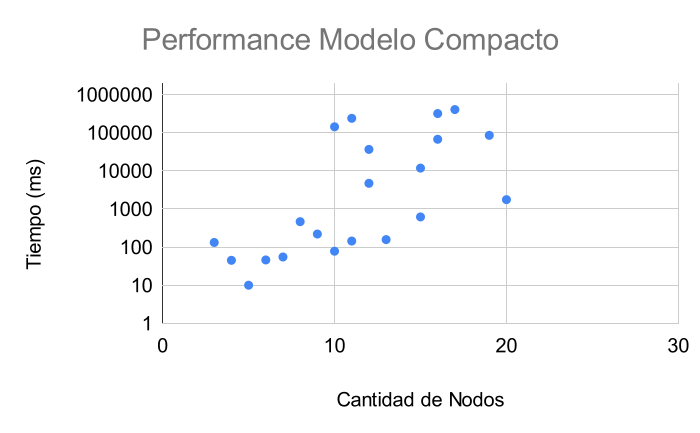
\includegraphics[width=\textwidth]{img/Performance Modelo Compacto.png}
         \caption{Modelo Compacto}
     \end{subfigure}
     \hfill
     \begin{subfigure}[b]{0.45\textwidth}
         \centering
         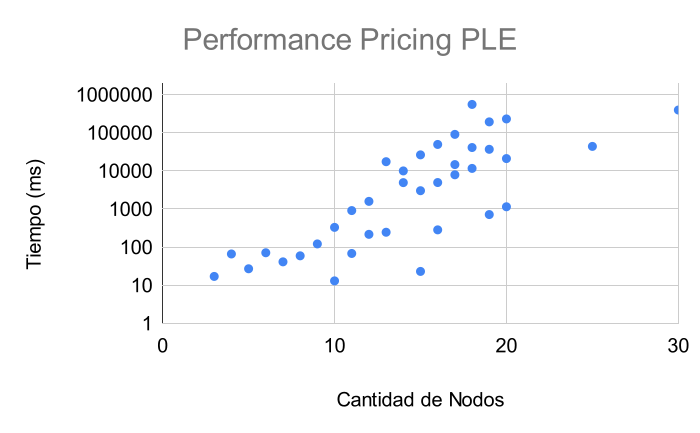
\includegraphics[width=\textwidth]{img/Performance Pricing PLE.png}
         \caption{Pricing con PLE}
     \end{subfigure}

     \begin{subfigure}[b]{0.45\textwidth}
         \centering
         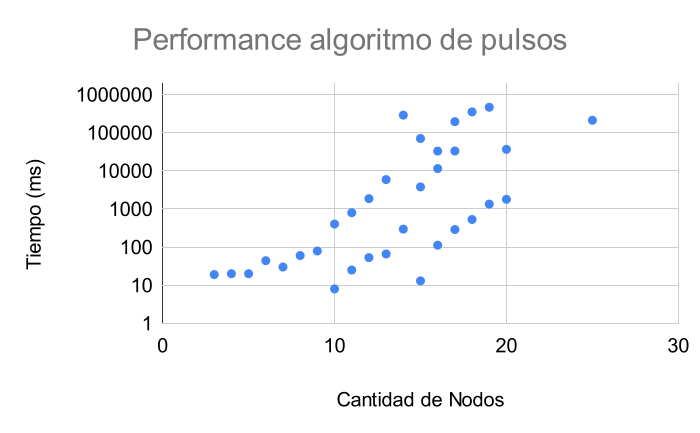
\includegraphics[width=\textwidth]{img/Performance algoritmo de pulsos.png}
         \caption{Pricing por pulsos}
     \end{subfigure}
     \hfill
     \begin{subfigure}[b]{0.45\textwidth}
         \centering
         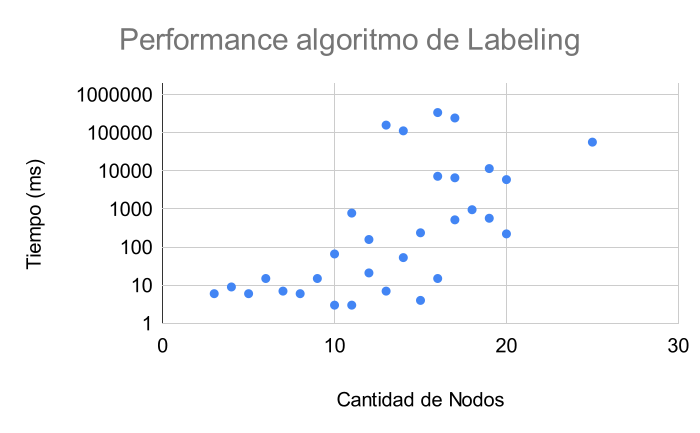
\includegraphics[width=\textwidth]{img/Performance algoritmo de Labeling.png}
         \caption{Label Setting}
     \end{subfigure}

        \caption{Tiempo vs. Cantidad de Nodos}
        \label{fig:performance-nodes}
\end{figure}

El próximo gráfico es muy similar pero ahora muestra la relación del tiempo con respecto a la cantidad de clientes en vez de nodos. La tendencia es muy parecida al caso anterior. Se podría discutir que en este caso el cúmulo de puntos se ajusta mejor a la linea que define la tendencia, que no sabemos calcular pero que demuestra el hecho de que la cantidad de clientes es una métrica un poco más fiel para predecir el tiempo total de ejecución. En la práctica sacar una conclusión de este estilo es demasiado fuerte y se sugiere fuertemente utilizar una combinación de ambos criterios.


\begin{figure}[H]
     \centering
     \begin{subfigure}[b]{0.45\textwidth}
         \centering
         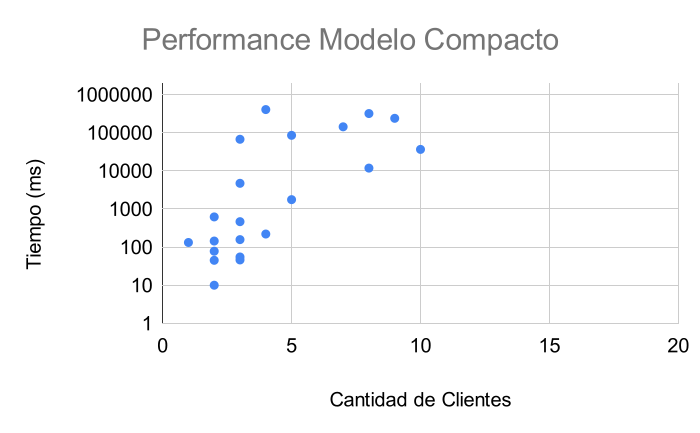
\includegraphics[width=\textwidth]{img/Performance Modelo Compacto (1).png}
         \caption{Modelo Compacto}
     \end{subfigure}
     \hfill
     \begin{subfigure}[b]{0.45\textwidth}
         \centering
         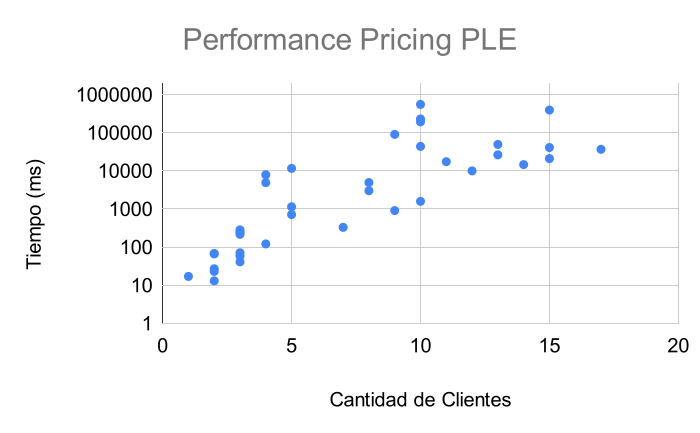
\includegraphics[width=\textwidth]{img/Performance Pricing PLE (1).png}
         \caption{Pricing con PLE}
     \end{subfigure}

     \begin{subfigure}[b]{0.45\textwidth}
         \centering
         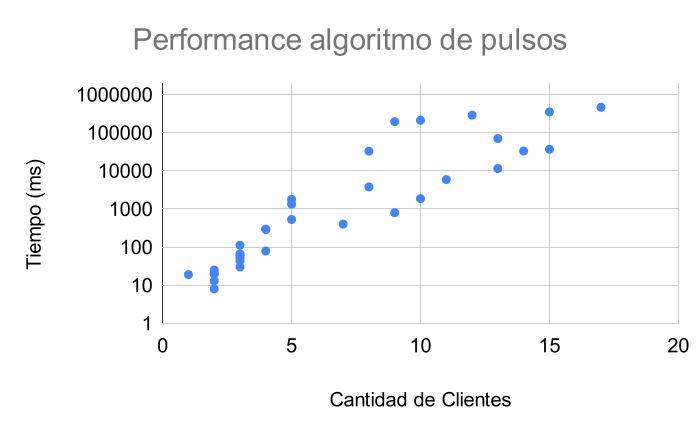
\includegraphics[width=\textwidth]{img/Performance algoritmo de pulsos (1).png}
         \caption{Pricing por pulsos}
     \end{subfigure}
     \hfill
     \begin{subfigure}[b]{0.45\textwidth}
         \centering
         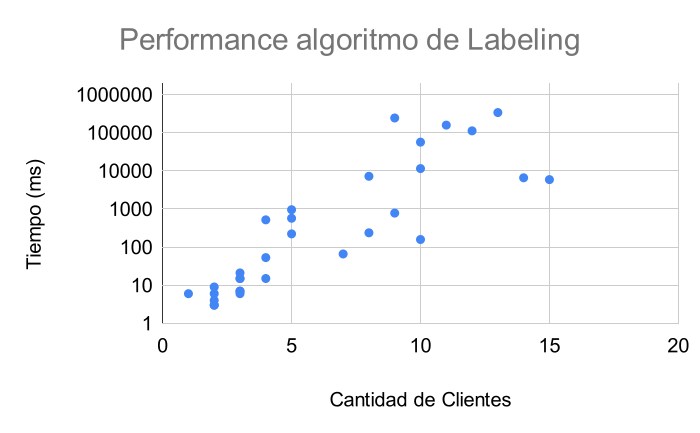
\includegraphics[width=\textwidth]{img/Performance algoritmo de Labeling (1).png}
         \caption{Label Setting}
     \end{subfigure}

        \caption{Tiempo vs. Cantidad de Clientes}
        \label{fig:performance-customers}
\end{figure}

\section{Heurísticas}

Un algoritmo de generación de columnas sin estar acompañado de Branch \& Price es una heurística en sí misma. Sin embargo, en esta sección nos referimos exclusivamente a heurísticas para resolver la relajación lineal, en particular que nos proveen una solución aproximada. 

El mecanismo que vamos a utilizar para realizar los experimentos va a ser en todos los casos el mismo: primero se corren en paralelo los algoritmos con y sin la heurística que se va a testear. Una métrica interesante sería la diferencia entre las soluciones de ambas variantes. Sin embargo, es de esperar que algunas instancias grandes solamente puedan ser corridas con el algoritmo aproximado, y por lo tanto para establecer una métrica de calidad de solución nos vamos a tener que conformar con la que veníamos utilizando hasta el momento, es decir, el gap contra el óptimo de la relajación lineal. Cabe aclarar que esta cota ahora tiene menos garantías, porque la relajación lineal también se resolvió de manera aproximada. Con esto como motivación, existen dos métricas de calidad de solución: una que mide el gap entre la solución exacta y la aproximada (es decir, la solución encontrada con y sin la heurística en cuestión) y otra para cuando no tiene una solución exacta, que mide la brecha entre la solución del Problema Maestro con y sin restricciones de integralidad (pero en ambos casos utilizando la heurística). Para no incurrir en redundancias, las columnas restantes son análogas a los experimentos anteriores.

\subsection{Heurísticas de Label Setting}
\label{section:experiments-label-setting-heur}

La heurística que se propone en la Sección \ref{subsubsection:segment-tree-heuristic}, donde se relajan las condiciones de dominación y eso permite hacer mucho más eficiente la estructura de datos que almacena las etiquetas y verifica si una domina a otra. Además esta estructura provee una cota superior a la cantidad de etiquetas almacenada que es mucho más ajustada que en el caso general. Otra ventaja que podemos sacar de esto es que el proceso que implica chequear si una etiqueta es dominada es más eficiente porque el \texttt{Segment Tree} tiene una complejidad logarítmica para operaciones de consulta. 

Todas estas características juntas producen tiempos mucho mejores, como se pueden explicar en la siguiente tabla. La mejora que produce esta heurística es sorprendente y sin dudas uno de los hallazgos importantes de esta tesis. El rendimiento mejora en casi la totalidad de las instancias y puede procesar muchos más clientes.

En este experimento naturalmente estamos comparando el algoritmo con las heurísticas que queremos analizar contra el algoritmo estándar que resuelve la relajación lineal a exactitud. Para cada uno de estos dos algoritmos, se registran el tiempo de ejecución y la cantidad de iteraciones de generación de columnas. La columna $\Delta$ hace referencia a la diferencia relativa entre los valores de la función objetivo en ambos algoritmos. Por otro lado, muchas veces no es posible calcular esta diferencia porque el algoritmo exacto no completó la ejecución y de esta manera no hay valor contra el cual comparar. Para esto agregamos una segunda columna que intenta dar una métrica de error, midiendo el gap con respecto a la cota inferior que veníamos utilizando hasta ahora, que es el valor objetivo en la relajación lineal.

\begin{landscape}


\begin{longtblr}[
  caption = {Comparación entre labeling exacto y aproximado},
]{
  colspec = {|lrrrrrrrrr|},
  rowhead = 1,
  hlines,
  row{even} = {gray9},
} 

Instancia    & \textbar{}N\textbar{} & \textbar{}S\textbar{} & \textbar{}K\textbar{} & T s/Heur. (ms)& \#Iter s/Heur.& T c/Heur. (ms)& \#Iter c/Heur.& $\Delta Fobj$& Gap
\\ 
\hline
n3\_s1\_k1   & 3                     & 1                     & 1                     & 238       & 1              & 4         & 1              & 0.00\%                   & 0.00\%      \\
n4\_s2\_k1   & 4                     & 2                     & 1                     & 18        & 4              & 22        & 4              & 0.00\%                   & 0.00\%      \\
n5\_s2\_k1   & 5                     & 2                     & 1                     & 25        & 4              & 25        & 4              & 0.00\%                   & 0.00\%      \\
n6\_s3\_k2   & 6                     & 3                     & 2                     & 55        & 4              & 50        & 4              & 0.00\%                   & 0.00\%      \\
n7\_s3\_k2   & 7                     & 3                     & 2                     & 29        & 3              & 12        & 3              & 0.00\%                   & 0.00\%      \\
n8\_s3\_k2   & 8                     & 3                     & 2                     & 47        & 4              & 28        & 4              & 0.00\%                   & 0.00\%      \\
n9\_s4\_k2   & 9                     & 4                     & 2                     & 44        & 4              & 27        & 4              & 0.00\%                   & 0.00\%      \\
n10\_s7\_k3  & 10                    & 7                     & 3                     & 161       & 6              & 46        & 6              & 0.00\%                   & 0.00\%      \\
n10\_s2\_k2  & 10                    & 2                     & 2                     & 9         & 1              & 3         & 1              & 0.00\%                   & 0.00\%      \\
n11\_s9\_k3  & 11                    & 9                     & 3                     & 851       & 11             & 47        & 9              & 6.82\%                & 0.00\%      \\
n11\_s2\_k2  & 11                    & 2                     & 2                     & 5         & 3              & 4         & 3              & 0.00\%                   & 0.00\%      \\
n12\_s10\_k3 & 12                    & 10                    & 3                     & 178       & 11             & 34        & 11             & 0.00\%                   & 0.00\%      \\
n12\_s3\_k2  & 12                    & 3                     & 2                     & 14        & 3              & 10        & 3              & 0.00\%                   & 0.00\%      \\
n13\_s3\_k2  & 13                    & 3                     & 2                     & 9         & 4              & 4         & 4              & 0.00\%                   & 0.00\%      \\
n13\_s11\_k3 & 13                    & 11                    & 3                     & 168685    & 14             & 105       & 14             & 0.00\%                   & 12.92\%  \\
n14\_s12\_k3 & 14                    & 12                    & 3                     & 110422    & 17             & 79        & 14             & 0.00\%                   & 4.35\%   \\
n14\_s4\_k2  & 14                    & 4                     & 2                     & 49        & 6              & 8         & 6              & 0.00\%                   & 0.00\%      \\
n15\_s2\_k2  & 15                    & 2                     & 2                     & 4         & 1              & 1         & 1              & 0.00\%                   & 0.00\%      \\
n15\_s13\_k4 & 15                    & 13                    & 4                     & TLE       & 19             & 117       & 17             & ---                   & 0.71\%   \\
n15\_s8\_k2  & 15                    & 8                     & 2                     & 269       & 12             & 37        & 12             & 0.00\%                   & 0.00\%      \\
n16\_s13\_k4 & 16                    & 13                    & 4                     & 345975    & 17             & 116       & 16             & 0.00\%                   & 0.51\%   \\
n16\_s8\_k2  & 16                    & 8                     & 2                     & 7034      & 14             & 33        & 11             & 0.00\%                   & 1.79\%   \\
n16\_s3\_k2  & 16                    & 3                     & 2                     & 16        & 4              & 5         & 4              & 0.00\%                   & 0.00\%      \\
n17\_s14\_k4 & 17                    & 14                    & 4                     & 6366      & 19             & 91        & 18             & 0.00\%                   & 0.84\%   \\
n17\_s4\_k2  & 17                    & 4                     & 2                     & 519       & 6              & 12        & 6              & 0.00\%                   & 0.00\%      \\
n17\_s9\_k2  & 17                    & 9                     & 2                     & 250728    & 18             & 113       & 18             & 0.00\%                   & 0.00\%      \\
n18\_s5\_k2  & 18                    & 5                     & 2                     & 945       & 5              & 61        & 5              & 0.00\%                   & 0.00\%      \\
n18\_s10\_k2 & 18                    & 10                    & 2                     & TLE       & 19             & 167       & 14             & ---                   & 0.00\%      \\
n18\_s15\_k4 & 18                    & 15                    & 4                     & TLE       & 18             & 158       & 18             & ---                   & 9.66\%   \\
n19\_s5\_k2  & 19                    & 5                     & 2                     & 545       & 8              & 20        & 7              & 0.00\%                   & 0.00\%      \\
n19\_s17\_k4 & 19                    & 17                    & 4                     & TLE       & 22             & 291       & 22             & ---                   & 3.26\%   \\
n19\_s10\_k2 & 19                    & 10                    & 2                     & 11219     & 17             & 78        & 15             & 0.00\%                   & 0.00\%      \\
n20\_s15\_k5 & 20                    & 15                    & 5                     & 5745      & 17             & 151       & 17             & 0.00\%                   & 4.17\%   \\
n20\_s10\_k2 & 20                    & 10                    & 2                     & TLE       & 17             & 225       & 17             & ---                   & 2.20\%   \\
n20\_s5\_k2  & 20                    & 5                     & 2                     & 213       & 7              & 13        & 7              & 0.00\%                   & 0.00\%      \\
n25\_s15\_k3 & 25                    & 15                    & 3                     & TLE       & 20             & 1094      & 20             & ---                   & 5.01\%   \\
n25\_s10\_k2 & 25                    & 10                    & 2                     & 55530     & 28             & 224       & 27             & 0.00\%                   & 0.00\%      \\
n25\_s20\_k5 & 25                    & 20                    & 5                     & TLE       & 24             & 7866      & 24             & ---                   & 10.59\%  \\
n30\_s20\_k3 & 30                    & 20                    & 3                     & TLE       & 34             & 3485      & 34             & ---                   & 3.82\%   \\
n30\_s15\_k2 & 30                    & 15                    & 2                     & TLE       & 27             & 982       & 27             & ---                   & 4.81\%   \\
n30\_s25\_k5 & 30                    & 25                    & 5                     & TLE       & 35             & 6467      & 35             & ---                   & 1.63\%   \\
n35\_s20\_k3 & 35                    & 20                    & 3                     & TLE       & 19             & 11450     & 32             & ---                   & 6.22\%   \\
n35\_s15\_k2 & 35                    & 15                    & 2                     & TLE       & 23             & 6244      & 29             & ---                   & 0.00\%      \\
n35\_s25\_k5 & 35                    & 25                    & 5                     & TLE       & 34             & 4612      & 34             & ---                   & 1.40\%   \\
n40\_s20\_k3 & 40                    & 20                    & 3                     & TLE       & 10             & 139188    & 60             & ---                   & 2.67\%   \\
n40\_s15\_k2 & 40                    & 15                    & 2                     & TLE       & 15             & 9243      & 34             & ---                   & 1.30\%   \\
n40\_s30\_k5 & 40                    & 30                    & 5                     & TLE       & 11             & 31271     & 40             & ---                   & 6.50\%   \\
n45\_s20\_k3 & 45                    & 20                    & 3                     & TLE       & 11             & 18615     & 30             & ---                   & 4.26\%   \\
n45\_s40\_k5 & 45                    & 40                    & 5                     & TLE       & 9              & 142394    & 64             & ---                   & 6.23\%   \\
n45\_s15\_k2 & 45                    & 15                    & 2                     & TLE       & 12             & 16576     & 34             & ---                   & 0.00\%      \\
n50\_s45\_k5 & 50                    & 45                    & 5                     & TLE       & 10             & 169553    & 83             & ---                   & 3.01\%   \\
n50\_s10\_k2 & 50                    & 10                    & 2                     & TLE       & 15             & 987       & 15             & ---                   & 0.00\%      \\
n50\_s20\_k3 & 50                    & 20                    & 3                     & TLE       & 11             & 33167     & 36             & ---                   & 2.75\%   \\
n55\_s20\_k3 & 55                    & 20                    & 3                     & TLE       & 8              & 28380     & 31             & ---                   & 3.97\%   \\
n55\_s10\_k2 & 55                    & 10                    & 2                     & TLE       & 17             & 4428      & 17             & ---                   & 5.09\%   \\
n55\_s45\_k5 & 55                    & 45                    & 5                     & TLE       & 9              & 422897    & 92             & ---                   & 2.36\%   \\
n60\_s10\_k2 & 60                    & 10                    & 2                     & TLE       & 8              & 8716      & 15             & ---                   & 7.90\%   \\
n60\_s20\_k3 & 60                    & 20                    & 3                     & TLE       & 7              & 172342    & 52             & ---                   & 1.54\%   \\
n60\_s50\_k5 & 60                    & 50                    & 5                     & TLE       & 4              & TLE       & 71             & ---                   & ---      \\
n65\_s10\_k2 & 65                    & 10                    & 2                     & TLE       & 15             & 5259      & 20             & ---                   & 0.00\%      \\
n65\_s20\_k3 & 65                    & 20                    & 3                     & TLE       & 9              & 95444     & 37             & ---                   & 0.00\%      \\
n65\_s55\_k5 & 65                    & 55                    & 5                     & TLE       & 6              & TLE       & 13             & ---                   & ---      \\
n70\_s10\_k2 & 70                    & 10                    & 2                     & TLE       & 5              & 46446     & 25             & ---                   & 5.56\%   \\
\hline
\end{longtblr}
\end{landscape}

Es alentador ver que hay muchas columnas con $\Delta Fobj = 0.00\%$; eso significa que la solución aproximada coincide con la exacta, por lo tanto, la heurística se dice que ``adivinó'' el verdadero valor del óptimo de la función objetivo. Lamentablemente no podemos extrapolar este resultado a instancias relativamente grandes porque el algoritmo exacto no termina la ejecución y por consiguiente tampoco podemos calcular la diferencia. 

Es claro que este es el algoritmo más rápido de los analizados, dado que permite procesar instancias mucho más grandes que los de secciones anteriores. Es digno de discusión si vale la pena sacrificar la garantía de exactitud (al menos para resolver la relajación lineal) para tener un gran incremento en rendimiento, incluso viendo que la pérdida de calidad de la solución no es muy grande en los casos que se pudo computar. Naturalmente no hay una respuesta universal y dependerá del caso de uso.


\subsection{2-Step Column Generation}
\label{section:2-step-cg-testing}

Las técnicas que se describen en \ref{section:2-step-cg} sirven para reducir marginalmente la cantidad de iteraciones de generación de columnas y en el caso de combinarse con un algoritmo aproximado, apunta a mejorar el valor de la función objetivo porque agrega a la base posibilidades que el pricing estándar desconoce. Con esto en mente, tiene sentido que la comparación de este experimento sea en base a un pricing aproximado, porque el efecto se aprecia mejor cuando hay muchas iteraciones. En esta subsección aplicamos la heurística de 2-Step Column Generation utilizando como pricing el algoritmo de Label Setting aproximado, es decir, ambas heurísticas al mismo tiempo. Es de esperar que en instancias chicas el overhead de aplicar este procedimiento dé tiempos más elevados, por lo tanto vale la pena solamente considerarlo a partir de cierto número de clientes. 

Cuando se mide el gap exacto, es decir, la diferencia porcentual entre la solución con y sin heurística respectivamente, el valor puede ser positivo o negativo, ya que se mide el incremento porcentual del valor con heurística con respecto al que no la aplica. Es decir, si el valor con heurística es menor al que no tiene heurística, este número será negativo. Como ambos entregan soluciones factibles, el que dé el menor valor estará más cerca del óptimo, y por lo tanto, en caso de que este algoritmo sea útil y 2-Step Column Generation mejore la solución, esperaríamos ver muchas columnas con valores negativos.

En la tabla que sigue medimos el tiempo en milisegundos tomado por los algoritmos con y sin esta mejora (en la columna ``T''), así como también la cantidad de iteraciones. Al igual que en el experimento anterior, se indican la diferencia entre los valores de la función objetivo entre dichas alternativas y el gap con respecto a la relajación lineal. 


\begin{landscape}
\begin{longtblr}[
  caption = {Comparación de Generación de Columnas con y sin 2-Step Column Generation},
]{
  colspec = {|lrrrrrrrrr|},
  rowhead = 1,
  hlines,
  row{even} = {gray9},
} 

Instancia    & \textbar{}N\textbar{} & \textbar{}S\textbar{} & \textbar{}K\textbar{} & T s/2GC (ms)& \#Iter s/2GC & T c/2GC (ms)& \#Iter c/2GC& $\Delta Fobj$& Gap
\\ 
\hline
n3\_s1\_k1   & 3                     & 1                     & 1                     & 130                 & 1                 & 3                   & 1                 & 0.00\%        & 0.00\%         \\
n4\_s2\_k1   & 4                     & 2                     & 1                     & 12                  & 4                 & 13                  & 4                 & 0.00\%        & 0.00\%         \\
n5\_s2\_k1   & 5                     & 2                     & 1                     & 9                   & 4                 & 10                  & 4                 & 0.00\%        & 0.00\%         \\
n6\_s3\_k2   & 6                     & 3                     & 2                     & 27                  & 4                 & 29                  & 3                 & 0.00\%        & 0.00\%         \\
n7\_s3\_k2   & 7                     & 3                     & 2                     & 14                  & 3                 & 10                  & 3                 & 0.00\%        & 0.00\%         \\
n8\_s3\_k2   & 8                     & 3                     & 2                     & 13                  & 4                 & 9                   & 4                 & 0.00\%        & 0.00\%         \\
n9\_s4\_k2   & 9                     & 4                     & 2                     & 17                  & 4                 & 14                  & 4                 & 0.00\%        & 0.00\%         \\
n10\_s7\_k3  & 10                    & 7                     & 3                     & 34                  & 6                 & 63                  & 7                 & 0.00\%        & 0.00\%         \\
n10\_s2\_k2  & 10                    & 2                     & 2                     & 3                   & 1                 & 2                   & 1                 & 0.00\%        & 0.00\%         \\
n11\_s9\_k3  & 11                    & 9                     & 3                     & 127                 & 9                 & 102                 & 11                & -6.38\%    & 0.00\%         \\
n11\_s2\_k2  & 11                    & 2                     & 2                     & 6                   & 3                 & 7                   & 3                 & 0.00\%        & 0.00\%         \\
n12\_s10\_k3 & 12                    & 10                    & 3                     & 76                  & 11                & 111                 & 11                & 0.00\%        & 0.00\%         \\
n12\_s3\_k2  & 12                    & 3                     & 2                     & 55                  & 3                 & 23                  & 3                 & 0.00\%        & 0.00\%         \\
n13\_s3\_k2  & 13                    & 3                     & 2                     & 8                   & 4                 & 6                   & 4                 & 0.00\%        & 0.00\%         \\
n13\_s11\_k3 & 13                    & 11                    & 3                     & 228                 & 14                & 97                  & 12                & 1.49\%     & 14.61\%     \\
n14\_s12\_k3 & 14                    & 12                    & 3                     & 88                  & 14                & 178                 & 21                & -5\%       & 7.55\%      \\
n14\_s4\_k2  & 14                    & 4                     & 2                     & 8                   & 6                 & 9                   & 6                 & 0.00\%        & 0.00\%         \\
n15\_s2\_k2  & 15                    & 2                     & 2                     & 2                   & 1                 & 2                   & 1                 & 0.00\%        & 0.00\%         \\
n15\_s13\_k4 & 15                    & 13                    & 4                     & 122                 & 17                & 138                 & 19                & 2.82\%     & 4.29\%      \\
n15\_s8\_k2  & 15                    & 8                     & 2                     & 33                  & 12                & 37                  & 11                & 0.00\%        & 0.00\%         \\
n16\_s13\_k4 & 16                    & 13                    & 4                     & 126                 & 16                & 125                 & 14                & 0.00\%        & 0.51\%      \\
n16\_s8\_k2  & 16                    & 8                     & 2                     & 38                  & 11                & 46                  & 10                & 0.00\%        & 1.79\%      \\
n16\_s3\_k2  & 16                    & 3                     & 2                     & 5                   & 4                 & 5                   & 4                 & 0.00\%        & 0.00\%         \\
n17\_s14\_k4 & 17                    & 14                    & 4                     & 84                  & 18                & 72                  & 15                & 0.00\%        & 0.84\%      \\
n17\_s4\_k2  & 17                    & 4                     & 2                     & 11                  & 6                 & 18                  & 6                 & 0.00\%        & 0.00\%         \\
n17\_s9\_k2  & 17                    & 9                     & 2                     & 109                 & 18                & 136                 & 15                & 0.00\%        & 0.00\%         \\
n18\_s5\_k2  & 18                    & 5                     & 2                     & 69                  & 5                 & 62                  & 9                 & 0.00\%        & 0.00\%         \\
n18\_s10\_k2 & 18                    & 10                    & 2                     & 166                 & 14                & 225                 & 16                & 3.45\%     & 0.00\%         \\
n18\_s15\_k4 & 18                    & 15                    & 4                     & 162                 & 18                & 214                 & 15                & -2.38\%    & 8.75\%      \\
n19\_s5\_k2  & 19                    & 5                     & 2                     & 21                  & 7                 & 12                  & 4                 & 0.00\%        & 0.90\%      \\
n19\_s17\_k4 & 19                    & 17                    & 4                     & 295                 & 22                & 220                 & 17                & 0.00\%        & 3.26\%      \\
n19\_s10\_k2 & 19                    & 10                    & 2                     & 81                  & 15                & 73                  & 15                & 0.00\%        & 0.00\%         \\
n20\_s15\_k5 & 20                    & 15                    & 5                     & 119                 & 17                & 84                  & 10                & 0.00\%        & 4.17\%      \\
n20\_s10\_k2 & 20                    & 10                    & 2                     & 214                 & 17                & 157                 & 15                & -7.06\%    & 0.00\%         \\
n20\_s5\_k2  & 20                    & 5                     & 2                     & 16                  & 7                 & 17                  & 7                 & 0.00\%        & 0.00\%         \\
n25\_s15\_k3 & 25                    & 15                    & 3                     & 1119                & 20                & 984                 & 20                & 2.29\%     & 7.20\%      \\
n25\_s10\_k2 & 25                    & 10                    & 2                     & 205                 & 27                & 181                 & 17                & 0.00\%        & 0.00\%         \\
n25\_s20\_k5 & 25                    & 20                    & 5                     & 7637                & 24                & 6437                & 24                & 0.00\%        & 10.50\%     \\
n30\_s20\_k3 & 30                    & 20                    & 3                     & 3377                & 34                & 4335                & 33                & -4.41\%    & 0.29\%      \\
n30\_s15\_k2 & 30                    & 15                    & 2                     & 1009                & 27                & 675                 & 25                & 1.02\%     & 5.10\%      \\
n30\_s25\_k5 & 30                    & 25                    & 5                     & 5937                & 35                & 4261                & 22                & 1.35\%     & 2.74\%      \\
n35\_s20\_k3 & 35                    & 20                    & 3                     & 10633               & 32                & 17403               & 28                & 0.00\%        & 6.02\%      \\
n35\_s15\_k2 & 35                    & 15                    & 2                     & 5955                & 29                & 9397                & 28                & -2.94\%    & 0.00\%         \\
n35\_s25\_k5 & 35                    & 25                    & 5                     & 4493                & 34                & 2894                & 27                & 0.55\%     & 1.68\%      \\
n40\_s20\_k3 & 40                    & 20                    & 3                     & 132799              & 60                & 58279               & 37                & 0.58\%     & 2.65\%      \\
n40\_s15\_k2 & 40                    & 15                    & 2                     & 9138                & 34                & 9148                & 36                & -5.15\%    & 0.00\%         \\
n40\_s30\_k5 & 40                    & 30                    & 5                     & 29496               & 40                & 33791               & 32                & -2.51\%    & 3.91\%      \\
n45\_s20\_k3 & 45                    & 20                    & 3                     & 17452               & 30                & 15749               & 29                & -4.40\%    & 0.00\%         \\
n45\_s40\_k5 & 45                    & 40                    & 5                     & 134447              & 64                & 151769              & 57                & -2.06\%    & 4.27\%      \\
n45\_s15\_k2 & 45                    & 15                    & 2                     & 16168               & 34                & 10852               & 26                & 0.00\%        & 0.00\%         \\
n50\_s45\_k5 & 50                    & 45                    & 5                     & 160539              & 83                & 87726               & 62                & 0.00\%        & 3.60\%      \\
n50\_s10\_k2 & 50                    & 10                    & 2                     & 963                 & 15                & 951                 & 14                & 0.00\%        & 1.20\%      \\
n50\_s20\_k3 & 50                    & 20                    & 3                     & 31134               & 36                & 13042               & 34                & -0.70\%    & 1.97\%      \\
n55\_s20\_k3 & 55                    & 20                    & 3                     & 27149               & 31                & 26015               & 26                & -0.46\%    & 3.90\%      \\
n55\_s10\_k2 & 55                    & 10                    & 2                     & 4277                & 17                & 4983                & 16                & 1.15\%     & 5.60\%      \\
n55\_s45\_k5 & 55                    & 45                    & 5                     & 399056              & 92                & 487636              & 76                & -0.42\%    & 4.94\%      \\
n60\_s10\_k2 & 60                    & 10                    & 2                     & 8588                & 15                & 10083               & 20                & 0.00\%        & 8.28\%      \\
n60\_s20\_k3 & 60                    & 20                    & 3                     & 165413              & 52                & 121311              & 29                & 6.70\%     & 4.77\%      \\
n60\_s50\_k5 & 60                    & 50                    & 5                     & TLE                 & 74                & TLE                 & 58                & ---        & ---         \\
n65\_s10\_k2 & 65                    & 10                    & 2                     & 5312                & 20                & 3883                & 13                & -29.66\%   & 0.00\%         \\
n65\_s20\_k3 & 65                    & 20                    & 3                     & 93359               & 37                & 199589              & 27                & 0.00\%        & 0.41\%      \\
n65\_s55\_k5 & 65                    & 55                    & 5                     & TLE                 & 13                & TLE                 & 10                & ---        & ---         \\
n70\_s10\_k2 & 70                    & 10                    & 2                     & 47371               & 25                & 33866               & 19                & 0.00\%        & 5.44\%      \\
\hline
\end{longtblr}
\end{landscape}


Dado que estamos corriendo 2-Step Column Generation por encima del conjunto de heurísticas que aplican al algoritmo de Label Setting (que son las mismas del experimento de la Sección \ref{section:experiments-label-setting-heur}), tiene sentido comparar estos resultados con los de dicha sección. Si bien el rendimiento en general no se ve sustancialmente beneficiado por esta nueva propuesta, vale la pena considerar una heurística como ésta porque cumple su objetivo inicial: la cantidad de iteraciones se ve reducida consistentemente. La calidad de la solución también mejora en un porcentaje sensible con respecto al experimento anterior y eso ayuda también a mejorar el error máximo esperado.


\subsection{Terminación temprana}

Un último experimento nos permite verificar el impacto de la heurística de terminación temprana. Como explicamos en la Sección \ref{section:finish-early}, estamos obligados a que el problema de pricing se resuelva a optimalidad. Resulta apropiado para esta prueba comparar ambos algoritmos (con y sin terminación temprana) utilizando como solver del problema de pricing el algoritmo por pulsos exacto. Respectivamente utilizamos las siglas ``c/TT'' y ``s/TT'' en las columnas de la siguiente tabla para inidicar que el algoritmo se corrió con y sin terminación temprana. 

En este caso, el valor que se eligió de para limitar el error es de $5\%$, a partir del cual se habilita la terminación temprana. Es discutible si este número es alto o no para instancias prácticas, pero a fines puramente teóricos queríamos tener un valor que evidencie sus propiedades.

Realmente solo tiene sentido comparar las entradas donde la cantidad de iteraciones se ve reducida, ya que en los otros casos la diferencia de tiempo se explica meramente en base a pequeñas diferencias usuales del entorno, y no por cuestiones inherentes al algoritmo. 

La fortaleza de esta heurística es que la degradación de la solución ya está acotada de antemano, pero la ganancia de tiempo no lo está. Idealmente, en instancias más grandes donde haya muchas iteraciones, se podría ver el verdadero efecto.

\begin{landscape}
\begin{longtblr}[
  caption = {Comparación de Generación de Columnas con y sin terminación temprana},
]{
  colspec = {|lrrrrrrrrr|},
  rowhead = 1,
  hlines,
  row{even} = {gray9},
} 

Instancia    & \textbar{}N\textbar{} & \textbar{}S\textbar{} & \textbar{}K\textbar{} & T s/TT (ms)& \#Iter s/TT& T c/TT (ms)& \#Iter c/TT& $\Delta Fobj$& Gap
\\ 
\hline
n3\_s1\_k1   & 3                     & 1                     & 1                     & 153                 & 1                 & 5                   & 1                 & 0.00\%        & 0.00\%         \\
n4\_s2\_k1   & 4                     & 2                     & 1                     & 53                  & 4                 & 34                  & 4                 & 0.00\%        & 0.00\%         \\
n5\_s2\_k1   & 5                     & 2                     & 1                     & 31                  & 4                 & 24                  & 4                 & 0.00\%        & 0.00\%         \\
n6\_s3\_k2   & 6                     & 3                     & 2                     & 92                  & 4                 & 94                  & 4                 & 0.00\%        & 33.33\%     \\
n7\_s3\_k2   & 7                     & 3                     & 2                     & 94                  & 3                 & 68                  & 3                 & 0.00\%        & 0.00\%         \\
n8\_s3\_k2   & 8                     & 3                     & 2                     & 130                 & 4                 & 52                  & 4                 & 0.00\%        & 0.00\%         \\
n9\_s4\_k2   & 9                     & 4                     & 2                     & 49                  & 4                 & 48                  & 4                 & 0.00\%        & 0.00\%         \\
n10\_s7\_k3  & 10                    & 7                     & 3                     & 287                 & 10                & 261                 & 10                & 0.00\%        & 0.00\%         \\
n10\_s2\_k2  & 10                    & 2                     & 2                     & 8                   & 1                 & 8                   & 1                 & 0.00\%        & 0.00\%         \\
n11\_s9\_k3  & 11                    & 9                     & 3                     & 825                 & 13                & 820                 & 13                & 0.00\%        & 0.00\%         \\
n11\_s2\_k2  & 11                    & 2                     & 2                     & 30                  & 3                 & 26                  & 3                 & 0.00\%        & 0.00\%         \\
n12\_s10\_k3 & 12                    & 10                    & 3                     & 1953                & 17                & 1936                & 17                & 0.00\%        & 0.00\%         \\
n12\_s3\_k2  & 12                    & 3                     & 2                     & 45                  & 4                 & 46                  & 4                 & 0.00\%        & 0.00\%         \\
n13\_s3\_k2  & 13                    & 3                     & 2                     & 65                  & 4                 & 62                  & 4                 & 0.00\%        & 0.00\%         \\
n13\_s11\_k3 & 13                    & 11                    & 3                     & 5985                & 20                & 6230                & 19                & 0.00\%        & 14.61\%     \\
n14\_s12\_k3 & 14                    & 12                    & 3                     & 299443              & 26                & 296396              & 26                & 0.00\%        & 4.35\%      \\
n14\_s4\_k2  & 14                    & 4                     & 2                     & 296                 & 7                 & 299                 & 7                 & 0.00\%        & 0.00\%         \\
n15\_s2\_k2  & 15                    & 2                     & 2                     & 13                  & 1                 & 13                  & 1                 & 0.00\%        & 0.00\%         \\
n15\_s13\_k4 & 15                    & 13                    & 4                     & 73893               & 25                & 71344               & 24                & 5.63\%     & 7.96\%      \\
n15\_s8\_k2  & 15                    & 8                     & 2                     & 3856                & 19                & 2953                & 14                & 0.00\%        & 0.00\%         \\
n16\_s13\_k4 & 16                    & 13                    & 4                     & 12021               & 21                & 10798               & 17                & 1.02\%     & 1.28\%      \\
n16\_s8\_k2  & 16                    & 8                     & 2                     & 35648               & 17                & 34967               & 15                & 0.00\%        & 12.05\%     \\
n16\_s3\_k2  & 16                    & 3                     & 2                     & 111                 & 5                 & 111                 & 5                 & 0.00\%        & 0.00\%         \\
n17\_s14\_k4 & 17                    & 14                    & 4                     & 34787               & 21                & 34796               & 21                & 0.00\%        & 6.58\%      \\
n17\_s4\_k2  & 17                    & 4                     & 2                     & 279                 & 5                 & 283                 & 5                 & 0.00\%        & 0.00\%         \\
n17\_s9\_k2  & 17                    & 9                     & 2                     & 208433              & 22                & 203256              & 20                & 3.17\%     & 2.09\%      \\
n18\_s5\_k2  & 18                    & 5                     & 2                     & 562                 & 8                 & 554                 & 8                 & 0.00\%        & 0.00\%         \\
n18\_s10\_k2 & 18                    & 10                    & 2                     & TLE                 & 13                & TLE                 & 13                & ---        & ---         \\
n18\_s15\_k4 & 18                    & 15                    & 4                     & 350970              & 24                & 347182              & 22                & 0.00\%        & 9.91\%      \\
n19\_s5\_k2  & 19                    & 5                     & 2                     & 1310                & 10                & 1168                & 9                 & 0.00\%        & 0.60\%      \\
n19\_s17\_k4 & 19                    & 17                    & 4                     & 468685              & 33                & 466743              & 30                & 0.00\%        & 6.27\%      \\
n19\_s10\_k2 & 19                    & 10                    & 2                     & TLE                 & 10                & TLE                 & 10                & ---        & ---         \\
n20\_s15\_k5 & 20                    & 15                    & 5                     & 36828               & 20                & 37086               & 20                & 0.00\%        & 13.10\%     \\
n20\_s10\_k2 & 20                    & 10                    & 2                     & TLE                 & 9                 & TLE                 & 9                 & ---        & ---         \\
n20\_s5\_k2  & 20                    & 5                     & 2                     & 1766                & 10                & 1467                & 8                 & 25.81\%    & 23.81\%     \\
n25\_s15\_k3 & 25                    & 15                    & 3                     & TLE                 & 5                 & TLE                 & 5                 & ---        & ---         \\
n25\_s10\_k2 & 25                    & 10                    & 2                     & 200226              & 34                & 178031              & 19                & 1.54\%     & 0.00\%         \\
\hline
\end{longtblr}
\end{landscape}
 


\cleardoublepage
\chapter{Conclusiones}

En este trabajo generalizamos la definición de \problem{Star Routing} que hace Tagliavini en \cite{tagliavini}. El problema que obtuvimos tiene una dificultad computacional categóricamente superior a la que suele existir en problemas de esta índole y por lo tanto se esperaba tratarlo para una cantidad de clientes mucho menor que en un paper donde se propone un algoritmo de estado del arte para resolver \problem{CVRP}. 

Primero definimos el Problema Maestro y el Problema Maestro Restringido en su forma genérica, y el algoritmo maestro de generación de columnas. Sobre esta base investigamos la literatura en cuanto a formulaciones eficientes del problema de pricing y tomamos tres de ellas, adaptándolas para el caso particular de \problem{Star VRP}.

El algoritmo estándar de pricing es un modelo de programación lineal que utilizamos como benchmark para comparar con los otros. Como inspiración en \cite{lozano-duque-medaglia} propusimos un algoritmo \emph{por pulsos}, un backtracking DFS, que resultó eficiente para resolver nuestra versión del \problem{ESPPRC}. El último enfoque, otro backtracking pero esta vez BFS, fue comprendido por algoritmo de labeling basado en el algoritmo de búsqueda mono-direccional propuesto en \cite{righini-salani}. 

Para reforzar los modelos introdujimos varias ideas en el frente heurístico. El algoritmo \emph{por pulsos} fue mejorado con el concepto de \emph{buckets de demanda} y con la mejora de la regla tradicional que denominamos \emph{multirollback}. Hasta donde tenemos conocimiento no existen publicaciones anteriores donde se propongan estas ideas. En paralelo, para el algoritmo de labeling se estudió una heurística eficiente de generar soluciones aproximadas que llamamos \emph{heurística de dominancia relajada} y otra heurística general de \emph{eliminación de simetría}.

Adicionalmente examinamos dos ideas que apuntan a mejorar el rendimiento del algoritmo de generación de columnas en sí mismo. Exploramos una idea clásica en la programación lineal que es \emph{early stopping}, y para eso ideamos una manera de acotar el óptimo de la relajación lineal por abajo, que cabe aclarar que no siempre se puede hacer. También con el objetivo de reducir el número de iteraciones del algoritmo, dimos a luz el concepto de \emph{2-Step Column Generation}, un conjunto de heurísticas un tanto peculiares que apuntan a reordenar el conjunto de clientes atendido ente los vehículos.


\section{Análisis de Resultados}

La hipótesis subyacente de este trabajo es que el modelo compacto es insuficiente para tratar problemas de ruteo de vehículos y por lo tanto utilizar un enfoque de generación de columnas puede reducir el tiempo de procesamiento notoriamente. Esta hipótesis se verifica en las instancias y condiciones en las que ejecutamos los experimentos.

El algoritmo de pricing más prometedor de este trabajo resultó ser el de labeling, ya que su performance en la versión exacta era competitiva con respecto a los otros, pero la versión aproximada permite calcular instancias considerablemente más grandes con una muy buena cota con respecto a la solución óptima. Además,  su implementación es bastante flexible ya que permite la adición de más reglas de dominancia, y fundamentalmente su complejidad cognitiva es menor que otros algoritmos con esquemas de acotación complejos.

El backtracking de búsqueda en profundidad, el que hasta ahora llamamos de \emph{pulsos} no presenta tiempos de ejecución significativamente mejores que el modelo estándar. Aparte de esto es difícil combinar con otras heurísticas clásicas, y tampoco hemos encontrado una manera de crear la versión aproximada.


\section{Discusión}

La dificultad adicional de poder atender o no un cliente cuando se pasa por una parada hace que el problema estudiado en esta tesis sea computacionalmente mucho más demandante y por lo tanto interesante. Parte del objetivo primigenio de este trabajo surge de la observación de que en el mundo fuera de la academia a menudo hay que lidiar con problemas que tienen pequeñas deformaciones con respecto a la versión ampliamente estudiada en la teoría, pero que lo convierten en un problema verdaderamente intratable, que apenas se puede concebir atacarlo en tiempo competitivo a través de heurísticas. En este caso, la dificultad aumenta por un factor importante ya que crece el espacio de soluciones factibles, y este hecho nos limita fuertemente la cantidad de clientes procesables.

Tomando las magnitudes que analizamos en la Sección \ref{section:complexity}, es un éxito haber podido correr una instancia de 70 nodos. Sin embargo este es un análisis superficial y no sirve para hacer predicciones acerca de la efectividad computacional real de los algoritmos. 

En términos coloquiales, lo que sucede que estamos resolviendo dos problemas independientes y por lo tanto la dificultad es la dificultad combinada de ambos. Primero tenemos el problema de encontrar una trayectoria viable que recorra el grafo y por otro lado el problema de asignar clientes que puedan ser atendidos desde esa trayectoria. Sin evitar un exceso de generalización, podemos relacionar esta idea con otros casos de la literatura donde se estudia la independencia de variables en modelos de programación lineal. Una cuestión que permanece abierta en este trabajo pero que sería muy interesante darle batalla es aplicar una técnica que nos permita atacar problemas que se pueden descomponer en varios ``subproblemas'' relacionados a los distintos tipos de variables. Una idea estándar que suele funcionar en un escenario similar es la descomposición combinatoria de Benders. En \cite{desrosiers2005primer} hay un excelente compendio sobre enfoques generalmente útiles para generación de columnas, y en particular se menciona el tema de formulaciones del Problema Maestro con variables independientes y por lo tanto problemas de pricing independientes, haciendo énfasis en si se puede explotar la estructura de bloques diagonal de la matriz. 


\section{Trabajo Futuro}

Creemos que este trabajo puede ser extendido en varias direcciones y esperamos haber planteado la duda para resolver cuestiones teóricas de fondo que escapan la formulación particular de este problema. Entre las ramas de investigación a futuro encontramos:

\begin{itemize}
    \item Sería especialmente relevante investigar cómo lidiar de manera eficiente con las variables independientes de este problema. Por ejemplo, reformulando el Problema Maestro de manera que existan múltiples clases de variables con varios problemas de pricing independientes, o bien aplicando algún tipo de técnica estándar como la descomposición de Benders.  

    \item Implementar un algoritmo de Branch \& Price que a priori nos permitiría obtener soluciones exactas del problema y no solamente el óptimo de la relajación lineal. Una idea válida es utilizar dos reglas de branching, una que se active cada vez que se visita un arco del grafo y otra por cada cliente visitado. Esta idea podría ser extendida aún más con la utilización de planos de corte y así constituyendo un Branch, Price \& Cut.
    
    \item Generalizar el algoritmo mono-direccional a uno de búsqueda bidireccional, que en la teoría es bastante utilizado.

    \item Pensar más reglas de dominancia y de pruning y probar matemáticamente que son válidas para descartar soluciones subóptimas.
        
    \item Combinar con otras heurísticas, entre las más populares están Decremental State Space Relaxation (DSSR) o Completion Bounds. 

    \item Proponer distintas formulaciones del Problema Maestro, en cuyo caso el problema de pricing será sustancialmente distinto, que nos permitan explotar mejor la independencia de variables.
    
\end{itemize}



%%%% BIBLIOGRAFIA
\backmatter
\bibliographystyle{plain}
\bibliography{tesis}

\end{document}
